\documentclass[12pt]{article}
\usepackage[utf8]{inputenc}
\usepackage[T1]{fontenc}
\usepackage{pdflscape} 
\usepackage{lmodern}
\usepackage[a4paper,bindingoffset=0.2in,%
            left=0.5in,right=0.5in,top=0.5in,bottom=1in,%
            footskip=.25in]{geometry}
\usepackage[colorlinks=true, linkcolor=Black, urlcolor=Blue]{hyperref}
\usepackage{graphicx}
\usepackage{subcaption}
\usepackage{listings}
\usepackage{color}
\usepackage[table]{xcolor}
\definecolor{lightgray}{gray}{0.9}

\definecolor{codegreen}{rgb}{0,0.6,0}
\definecolor{codegray}{rgb}{0.5,0.5,0.5}
\definecolor{codepurple}{rgb}{0.58,0,0.82}
\definecolor{backcolour}{rgb}{0.95,0.95,0.92}

\lstdefinestyle{mystyle}{
	backgroundcolor=\color{backcolour},   
	commentstyle=\color{codegreen},
	keywordstyle=\color{magenta},
	numberstyle=\tiny\color{codegray},
	stringstyle=\color{codepurple},
	basicstyle=\ttfamily\footnotesize,
	breakatwhitespace=false,         
	breaklines=true,                 
	captionpos=b,                    
	keepspaces=true,                 
	numbers=left,                    
	numbersep=5pt,                  
	showspaces=false,                
	showstringspaces=false,
	showtabs=false,                  
	tabsize=2
}


\begin{document}
\title{Sprawozdanie z zadania na Informatykę w Medycynie\\
\large Wykrywanie naczyń dna siatkówki oka\\
\large Sebastian Michoń 136770, Patryk Jedlikowski 136723}
\date{\vspace{-10ex}}
\maketitle

\section{Wstęp}
Dane są 3 różne notebooki
\begin {enumerate}
\item Basic\_version.ipynb - rozwiązanie na 3.0 - baseline model, wykorzystujący podstawowe techniki przetwarzania obrazów, w tym operacje morfologiczne.
\item kNN\_version.ipynb - rozwiązanie na 4.0 - wersja, która wykorzystuje podobieństwo (odleglość) obserwacji w zbiorze testowym do obserwacji ze zbioru treningowego do przyporządkowania elementu ze zbioru testowego do odpowiedniej klasy. Skorzystano tutaj z wariancji kolorów i momentów centralnych
\item Random\_forest.ipynb - rozwiązanie na 5.0 - wersja używa podzbioru obserwacji do stworzenia jednego drzewa - "silnego predyktora" (strong learner), po stworzeniu 50 drzew i procesie trenowania ich używane są one do stwierdzenia, czy dany fragment obrazu jest naczyniem krwionośnym. Do Hyperparameter Tuningu (Znalezienie najlepszej maksymalnej wartości głębokości drzewa) użyta została k-krotna skrośna walidacja.
\end {enumerate}

\section{Model podstawowy}
\begin {enumerate}
	\item Wczytywany jest obraz w czerni i bieli (w kolejnych wersjach algorytmu - kNN i Random forest - to się zmieni)
	\item Wstępne przetwarzanie składa się z: normalizacji histogramu kolorów, denoisingu (który ma praktycznie zerowy wpływ na jakość predykcji) oraz 11-krotnego poddania obrazu wpływowi kernela Gaussa (blura, 5*5) - dzięki temu obraz jest dużo bardziej rozmyty, co ułatwi znalezienie tylko interesujących z perspektywy zadania krawędzi.
	\item Właściwe przetwarzanie obrazu to użycie filtra prewitta do wyróżnienia wszystkich krawędzi, które później, w końcowej fazie będę modyfikował.
	\item Końcowa faza przetwarzania to, kolejno:
	\begin{enumerate}
		\item Nałożenie zerodowanej maski na powstały obraz: erozja rozszerzy czarną przestrzeń (obwódkę) maski, następnie wykonana zostanie operacja logicznego \& na rozszerzonej masce i obrazie powstałym po użyciu filtra krawędziowego. Dzięki temu usunę z obrazu po filtrowaniu krawędzie na zetknięciu maski z właściwym obrazem.
		\item Usunięcie wykrytych krawędzi tam, gdzie obraz jest najjaśniejszy - dzięki temu usunę białą plamkę widoczną na każdym obrazie z końcowego efektu przetwarzania. Opiera się to na thresholdingu: usuwam krawędzie tam, gdzie stopień jasności jest wyższy niż \(\frac{2}{3}\) maksymalnej jasności obrazu (czyli wyższy niż 165).
		\item Dokonuję kolejno morfologicznego domknięcia i erozji obrazu. Dzięki temu grubość krawędzi na obrazie wynikowym zostanie zmniejszona, ponadto zostaną one wypełnione od wewnątrz
	\end{enumerate}
	\item Do ewaluacji algorytmu użyłem średniej geometrycznej miar: precision i recall. Srednia geometryczna była wygodniejsza od arytmetycznej, ponieważ mocniej zaniżała oszacowaną skuteczność algorytmu, jeśli jedno z recall/precision było bliskie 0. Dla 20 przetwestowanych obrazów z zestawu średnia średnich geometrycznych tych miar to 0.5729099817180116.
\end {enumerate}

\section{Klasyfikator odległościowy}
\begin{enumerate}
	\item Wczytywany jest obraz zarówno w czerni i bieli, jak i w kolorze
	\item Nie dokonano wstępnego przetwarzania, ponieważ nie prowadziło ono do zwiększenia skuteczności, wręcz przeciwnie - usunięcie normalizacji histogramu kolorów zwiększyło średnią geometryczną precision i recall o 15 punktów procentowych. Być może wynika to z większego rozrzutu miar, a co za tym idzie mniejszej użyteczności wariancji.
	\item Aby wytrenować algorytm, wybrany został podzbiór punktów jednego obrazu. Podzbiór był wybierany w taki sposób, że:
	\begin{enumerate}
		\item Losuję koordynaty \(x, y\) pojedynczego punkt z obrazu.
		\item Jeśli koordynaty te należą do punktu, który nie został jeszcze wybrany i nie należy do maski to zostaje dodany do zbioru wybranych punktów jeśli jest on naczyniem krwionośnym, albo losowo wybrana liczba całkowita z przedziału \(x \in <0;3>: x \equiv 0\ (mod\ 4)\). Dzięki temu liczba wybranych punktów b z obu klas będzie bardziej zrównoważona, bo na 10 wylosowanych par liczb około jedna reprezentuje naczynie krwionośne.
		\item Dla wybranego zbioru punktów znajdowana jest informacja o punkcie, w tym: intensywność kolorów w punkcie, wariancje kolorów w obrazie o rozmiarze 10*10, którego centrum jest ten obraz (używany jest padding, aby każdy podobraz mógł uzyskać takie informacje), a także jego momenty centralne. Nie używałem momentów Hu, ponieważ spowalniały one proces predykcji nie zwiększając skuteczności algorytmu.
		\item Dla wybranego zbioru punktów znajdowana jest także informacja o wartośći maski eksperckiej (z naczyniami krwionośnymi) w tym punkcie.
		\item Przed treningiem dokonana zostaje normalizacja zbioru testowego - bez niej algorytm osiąga takie same rezultaty, ale proces trenowania i predykcji wykonuje się około 10 razy wolniej. Wagi dla poszczególnych zmiennych są takie same.
		\item Algorytm jest trenowany na wybranych danych.
	\end{enumerate}
	\item Analogicznie wybierany jest zbiór informacji do testowanego obrazu. W ramach testowania w analogiczny sposób do poprzedniego zadania porównywany jest rezultat treningu z maską ekspercką. Rezultaty są podobne do tych z zadania poprzedniego, przy czym zmniejsza się accuracy - które nie używa w tym algorytmie punktów spoza maski  obiektywu - przy czym ta miara i tak nie była używana do szacowania jakości algorytmu. Punkty z maski zawsze były klasyfikowane jako true negative, co nie ma wpływu ani na precision, ani recall.
\end{enumerate}


\section{Las drzew losowych}
\begin{enumerate}
	\item Proces wstępnego przetwarzania (czyli jego brak) i wybór punktów jednego obrazu jest analogiczny. Różnicą jest występowanie hyperparameter tuningu używającego k-krotnej skrośnej walidacji i ternary searcha, a także proces treningu.
	\item Trening odbywa się na wybranych punktach z 3 różnych obrazów, ręcznie wybranych, które były relatywnie niepodobne do siebie - dzięki temu możliwe było pokrycie całego zbioru testowego ze średnią geometryczną precision i recall nie mniejszą niż 0.5 dla wszystkich obrazów.
	\item Co ciekawe, obrazy poddane preprocessingowi ponownie osiągały niższą średnią średnich geometrycznych (o ok. 0.02) - tym razem jednak była ona spowodowana tym, że o ile większość obrazów miała wyższą średnią geometryczną recall i precision, o tyle kilka spadło gwałtownie - w szczególności, obrazek 11. z zestawu dr spadł o ponad 0.25, co obiżyło średnią średnich geometrycznych o ponad 0.01.
	\item K-skrośna walidacja została użyta do hyperparameter tuningu: z wybranego zestawu treningowego wyodrębniane są losowo 4 zbiory, następnie dla danych \(a, b\) 4 drzewa są trenowane na 3 grupach i testowane na 4., każde drzewo testowane na innej z 4 grup. \(a, b\) oznaczają maksymalną głębokość drzewa: zakładane jest, że zależność precyzji drzewa od głębokości jest najpierw niemalejąca (im większa głębokość, tym wyższa precyzja - drzewo o głębokości 2 uchwyci więcej informacji niż drzewo o głębokości 1), następnie nierosnąca (im większa głębokość, tym większa złożoność pamięciowa i tym więcej zbędnych informacji zapamiętuje drzewo - gdyby nie operowanie na lesie, a nie pojedynczym drzewie, niechybnie zaszedłby overfitting). To daje podstawy do użycia ternary searcha - szukam dla przedziału \(<l;r>\)
\end{enumerate}




\section{Tablica wynków: kody sit i pierwiastkowe}
Oznaczenia i skróty:
\begin{enumerate}
	\item name - nazwa kodu, pierwsze cyfry jego nazwy i skrót.
	\item left, right - przedział, dla którego wykonano program.
	\item T - liczba wątków
	\item Elapsed - czas, który upłynął od początku przetwarzania
	\item Ticks - liczba cykli procesora w trakcie wykonywania kodu.
	\item IR - Instructions Retired
	\item R - Retired
	\item FEB, BEB - Front-end bound, Back-end Bound
	\item MB, CB - Memory Bound,  Core Bound
	\item L1, L2, L3 - L1 Bound, L2 Bound, L3 Bound
	\item DRB, DTB - DRAM Bound, DTLB Store Overhead
	\item ECPU - Effective CPU Utilization
	\item Div - przyspieszenie przetwarzania równoległego
	\item Eff - efektywność przetwarzania równoległego
	\item Avg - liczba przetestowanych liczb w jednostce czasu.
\end{enumerate}
\begin{flushleft}
\begin{landscape}
		\rowcolors{2}{gray!25}{white}
		\captionof{table}{Efektywność i parametry wykonania poszczególnych programów}
		\resizebox{\columnwidth}{!}{%
		\begin{tabular}{| l | l | l | l | l | l | l | l | l | l | l | l | l | l | l | l | l | l | l | l | l |}
			\rowcolor{gray!50}
			\hline
			name & left & right & T & Elapsed[\(s\)] & Ticks & IR & R[\(\%\)] & FEB[\(\%\)] & BEB[\(\%\)] & MB[\(\%\)] & CB[\(\%\)] & L1[\(\%\)] & L2[\(\%\)] & L3[\(\%\)] & DRB[\(\%\)] & DTB[\(\%\)] & ECPU[\(\%\)] & Div & Eff & Avg[\(\frac{1}{s}\)] \\ \hline
			01\_es & 2 & 1.00E+09 & 1 & 10.312 & 4.38E+10 & 1.36E+10 & 7.2 & 0.4 & 92.2 & 76.4 & 15.8 & 18.5 & 0.2 & 9.2 & 0.0 & 30.7 & 24.2 & 1.0 & 1.0 & 9.70E+07 \\ \hline
			03\_efss & 2 & 1.00E+09 & 2 & 10.448 & 4.96E+10 & 1.44E+10 & 6.8 & 0.4 & 92.5 & 76.8 & 15.7 & 16.3 & 0.0 & 12.1 & 0.0 & 32.7 & 27.2 & 0.99 & 0.49 & 9.57E+07 \\ \hline
			03\_efss & 2 & 1.00E+09 & 4 & 10.094 & 6.11E+10 & 1.62E+10 & 7.4 & 0.3 & 91.9 & 74.7 & 17.2 & 7.8 & 0.0 & 18.8 & 0.0 & 37.5 & 34.8 & 1.02 & 0.26 & 9.91E+07 \\ \hline
			04\_efhs & 2 & 1.00E+09 & 2 & 10.026 & 5.85E+10 & 1.22E+10 & 4.4 & 0.8 & 94.7 & 78.2 & 16.5 & 6.2 & 1.2 & 20.3 & 0.0 & 36.4 & 33.3 & 1.03 & 0.51 & 9.97E+07 \\ \hline
			04\_efhs & 2 & 1.00E+09 & 4 & 8.666 & 1.14E+11 & 1.43E+10 & 2.9 & 0.9 & 95.8 & 78.0 & 17.8 & 0.0 & 0.3 & 29.4 & 0.0 & 41.8 & 77.8 & 1.19 & 0.30 & 1.15E+08 \\ \hline
			05\_efds & 2 & 1.00E+09 & 2 & 7.417 & 6.24E+10 & 1.39E+10 & 5.3 & 0.7 & 93.8 & 76.8 & 17.0 & 19.0 & 0.2 & 9.6 & 0.0 & 35.5 & 48.1 & 1.39 & 0.70 & 1.35E+08 \\ \hline
			05\_efds & 2 & 1.00E+09 & 4 & 6.654 & 1.07E+11 & 1.47E+10 & 3.2 & 0.9 & 95.5 & 78.3 & 17.2 & 5.9 & 0.2 & 22.3 & 0.0 & 35.7 & 95.7 & 1.55 & 0.39 & 1.50E+08 \\ \hline
			07\_ed & 2 & 1.00E+09 & 1 & 11.037 & 4.68E+10 & 1.91E+10 & 9.2 & 0.9 & 89.7 & 72.9 & 16.7 & 19.8 & 2.6 & 10.0 & 0.0 & 34.7 & 24.2 & 0.93 & 0.93 & 9.06E+07 \\ \hline
			07\_ed & 2 & 1.00E+09 & 2 & 9.801 & 8.25E+10 & 1.97E+10 & 5.3 & 0.6 & 93.9 & 73.2 & 20.7 & 8.2 & 0.0 & 0.0 & 22.6 & 36.6 & 48.1 & 1.05 & 0.53 & 1.02E+08 \\ \hline
			07\_ed & 2 & 1.00E+09 & 4 & 9.013 & 1.45E+11 & 1.96E+10 & 3.9 & 0.5 & 95.4 & 72.8 & 22.6 & 18.7 & 0.0 & 11.2 & 0.0 & 33.8 & 95.5 & 1.14 & 0.29 & 1.11E+08 \\ \hline
			08\_esd & 2 & 1.00E+09 & 1 & 1.498 & 6.33E+09 & 1.79E+10 & 49.2 & 14.4 & 26.2 & 20.4 & 5.8 & 19.5 & 4.7 & 1.7 & 0.0 & 1.8 & 24.2 & 6.88 & 6.88 & 6.68E+08 \\ \hline
			08\_esd & 2 & 1.00E+09 & 2 & 0.775 & 6.35E+09 & 1.79E+10 & 49.2 & 12.0 & 29.0 & 20.1 & 8.8 & 18.8 & 1.4 & 1.1 & 0.0 & 1.2 & 47.2 & 13.31 & 6.65 & 1.29E+09 \\ \hline
			08\_esd & 2 & 1.00E+09 & 4 & 0.429 & 6.50E+09 & 1.80E+10 & 57.6 & 10.8 & 20.0 & 12.2 & 7.8 & 17.5 & 0.0 & 2.3 & 0.0 & 0.9 & 90.7 & 24.04 & 6.01 & 2.33E+09 \\ \hline
			09\_sd & 2 & 1.00E+07 & 1 & 3.84 & 1.60E+10 & 1.76E+10 & 46.4 & 41.5 & 11.6 & 8.4 & 3.2 & 26.3 & 0.0 & 0.0 & 0.0 & 0.0 & 24.9 & - & 2.69 & 2.60E+06 \\ \hline
			09\_sd & 2 & 1.00E+07 & 4 & 1.291 & 1.98E+10 & 2.16E+10 & 39.0 & 28.1 & 31.6 & 28.1 & 3.5 & 21.4 & 0.0 & 0.0 & 0.0 & 0.1 & 91.2 & - & 2.00 & 7.75E+06 \\ \hline
	\end{tabular}
}\end{landscape}
\end{flushleft}

\begin{figure}[h!]
	\centering
	\begin{subfigure}[b]{0.32\linewidth}
		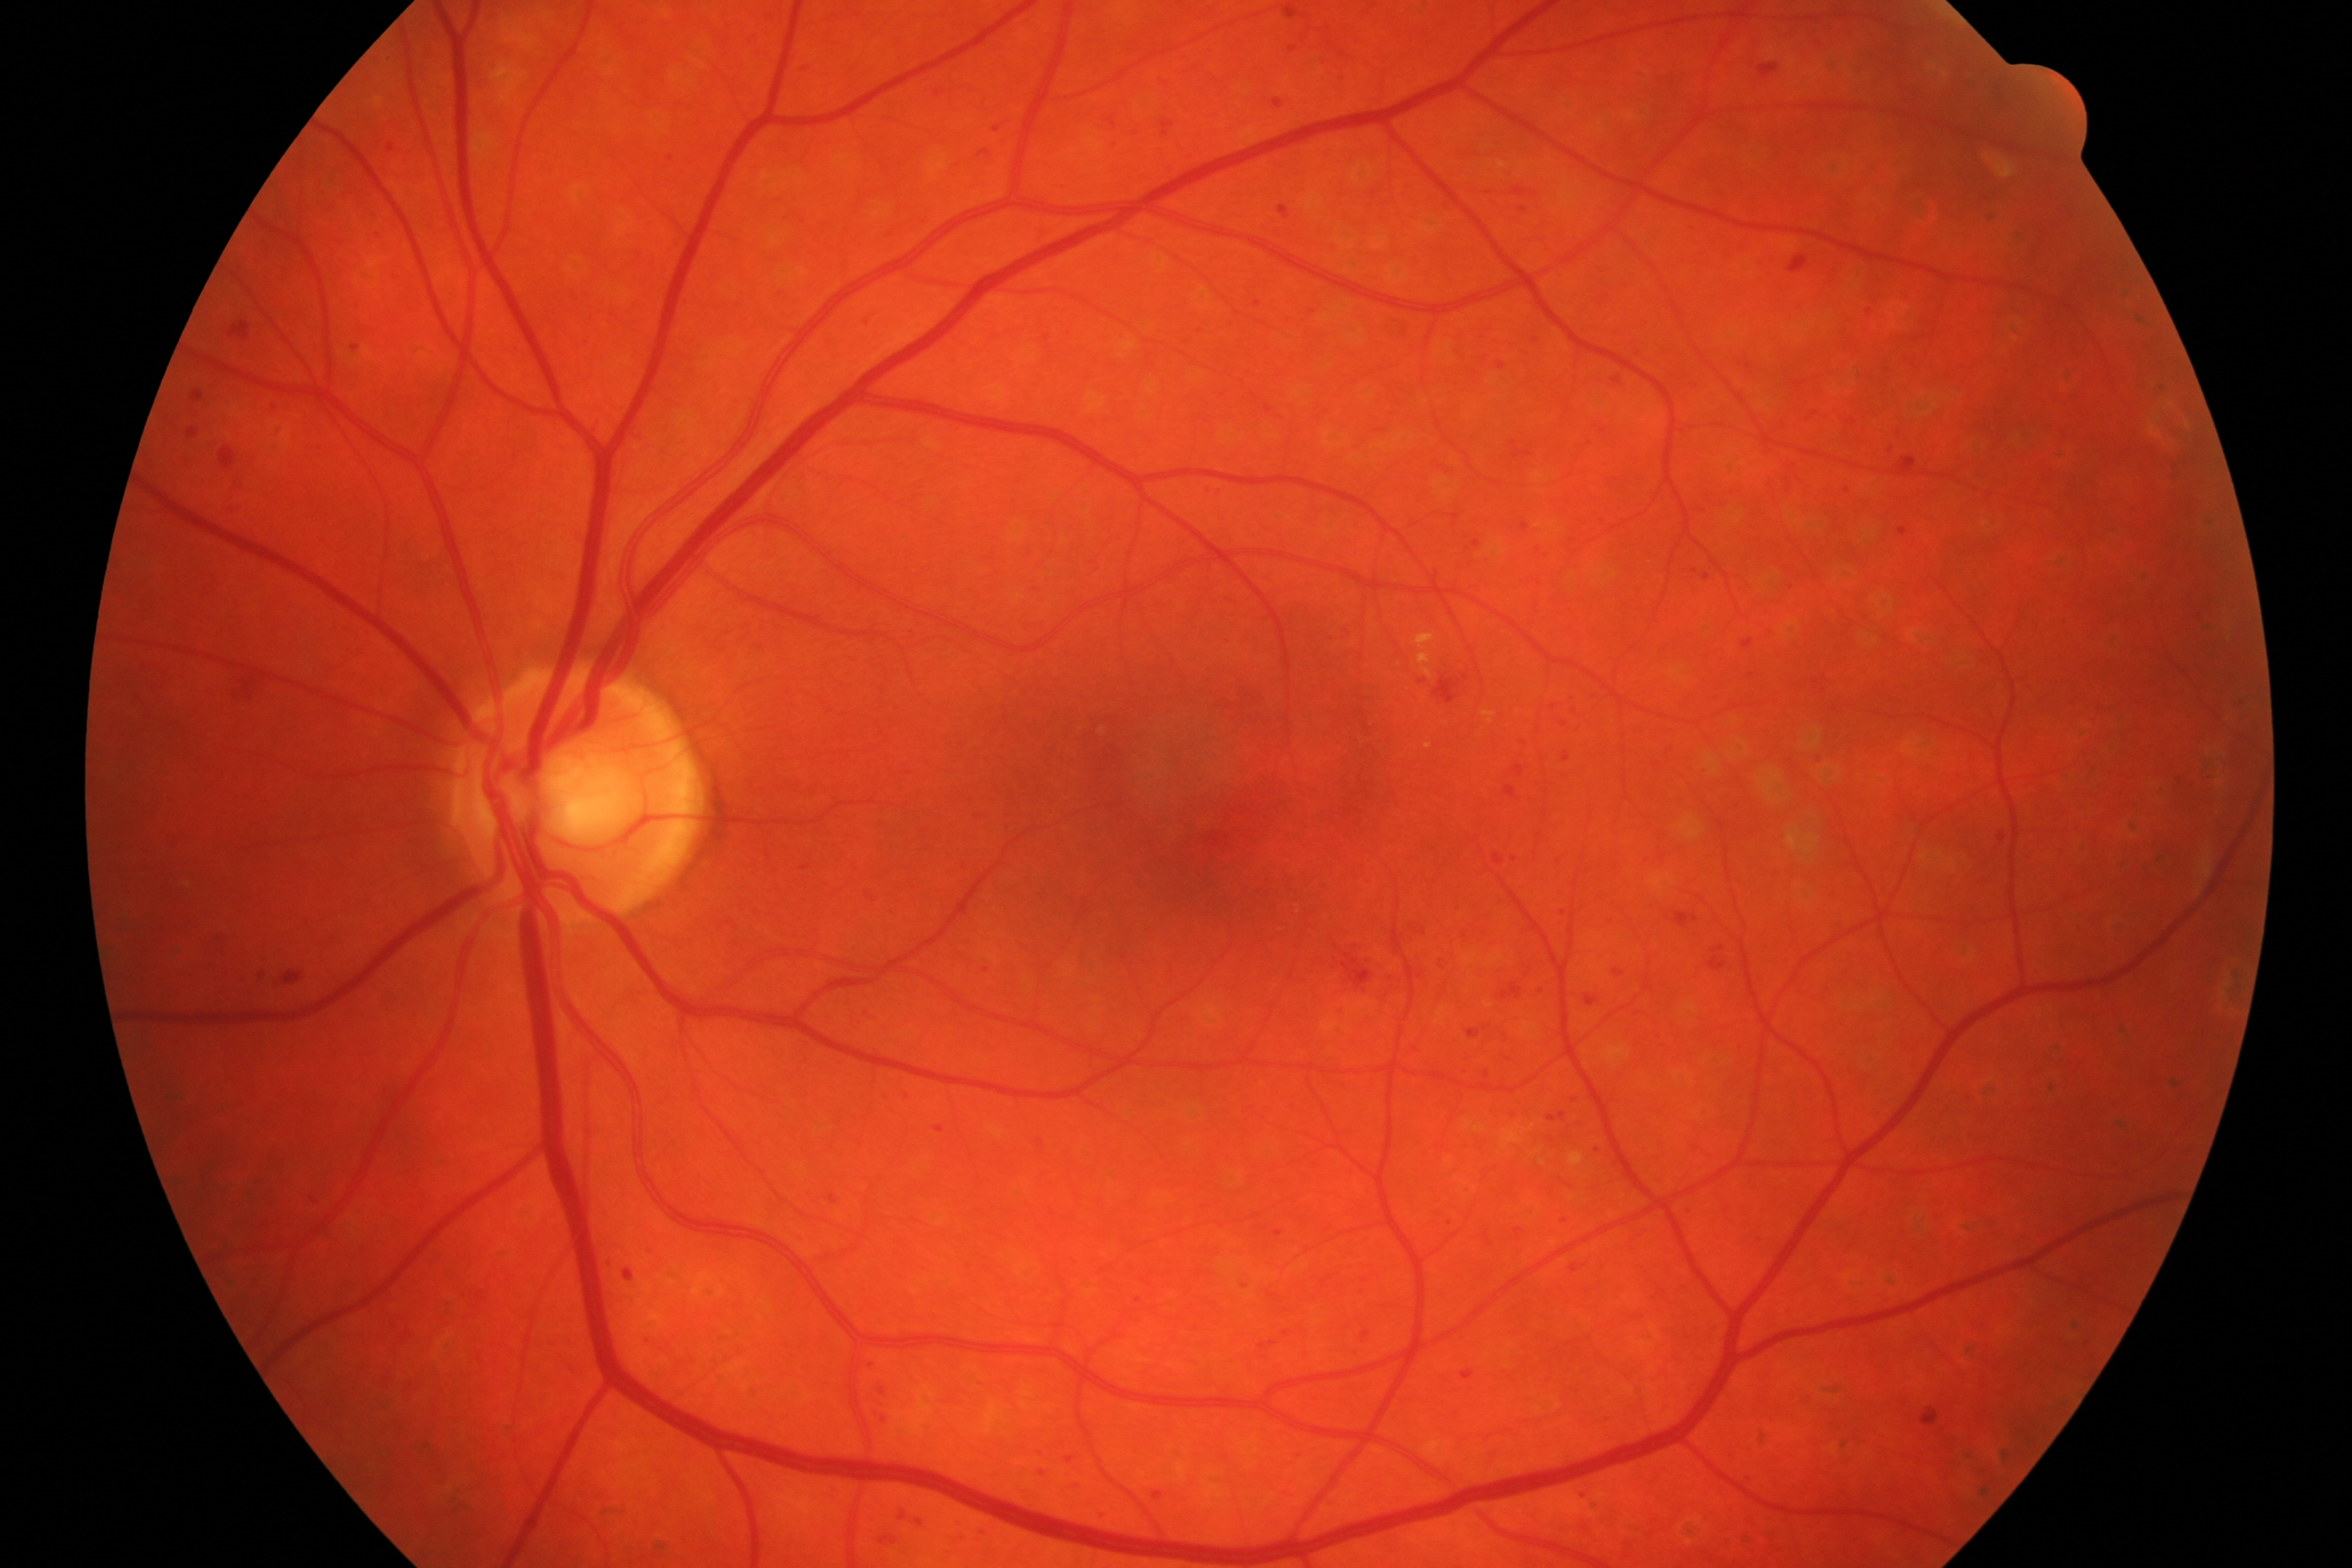
\includegraphics[width=\linewidth]{images/01_dr.jpg}
	\end{subfigure}
	\begin{subfigure}[b]{0.32\linewidth}
		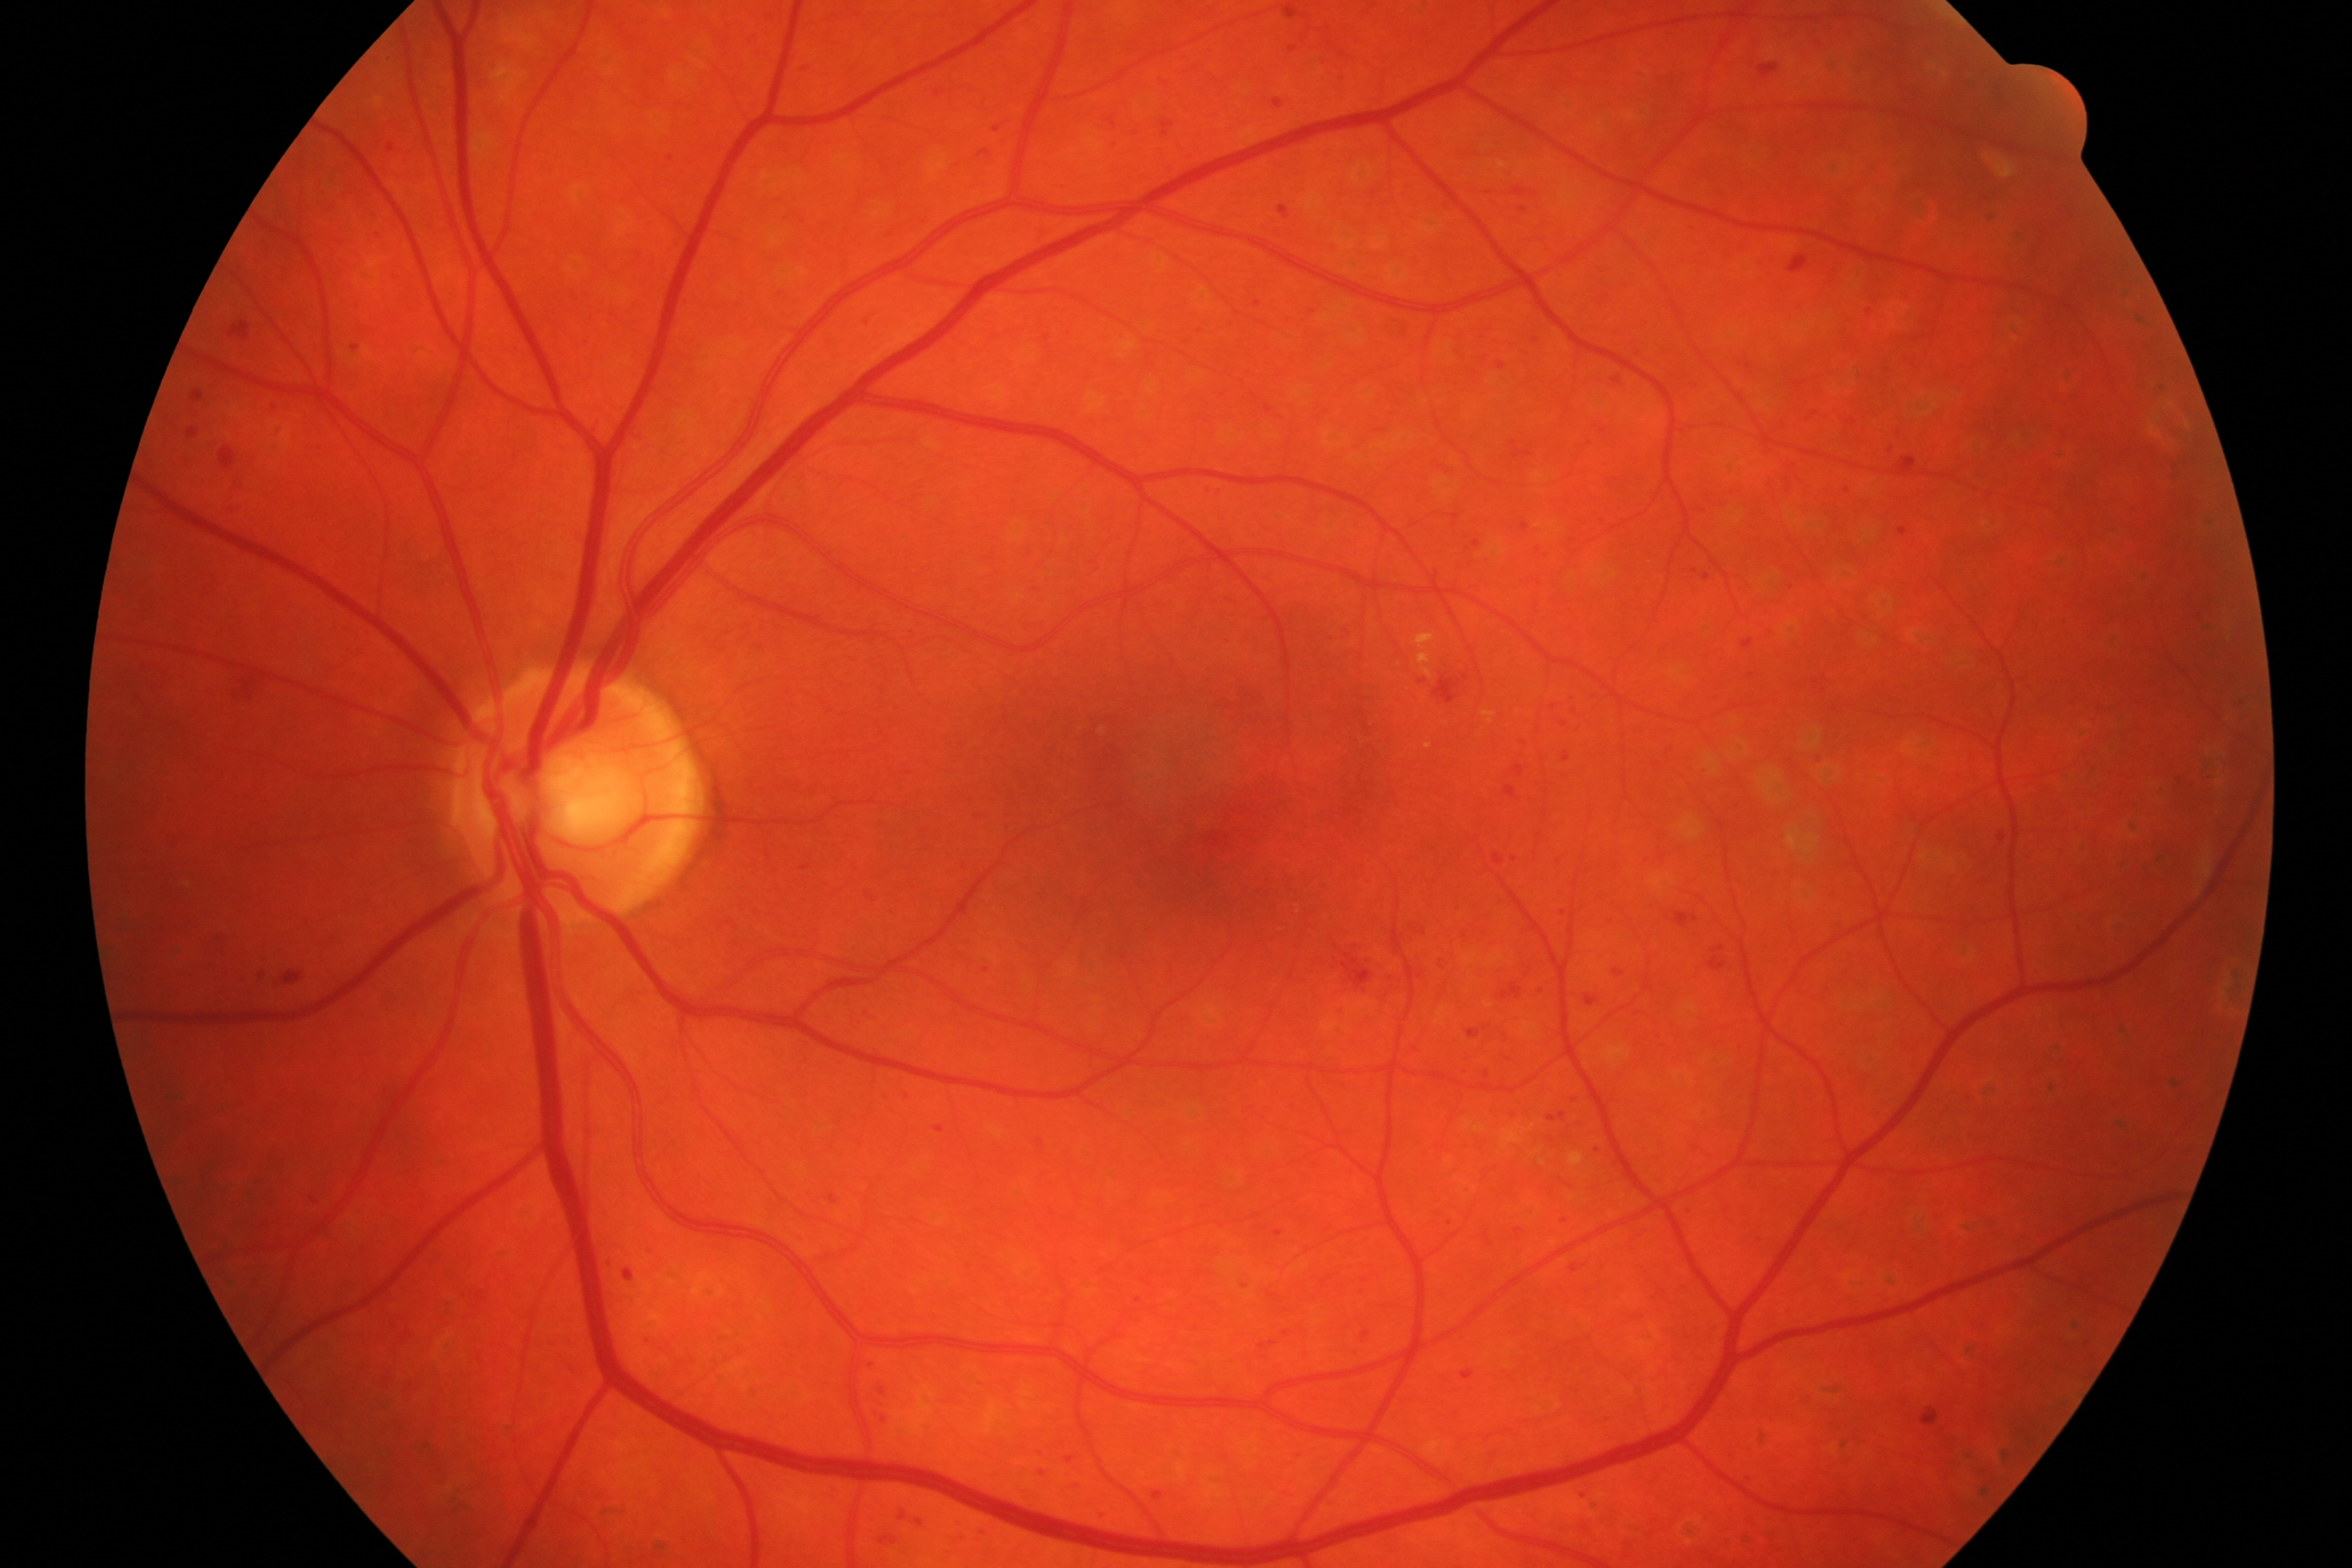
\includegraphics[width=\linewidth]{images/01_dr.jpg}
	\end{subfigure}
	\begin{subfigure}[b]{0.32\linewidth}
		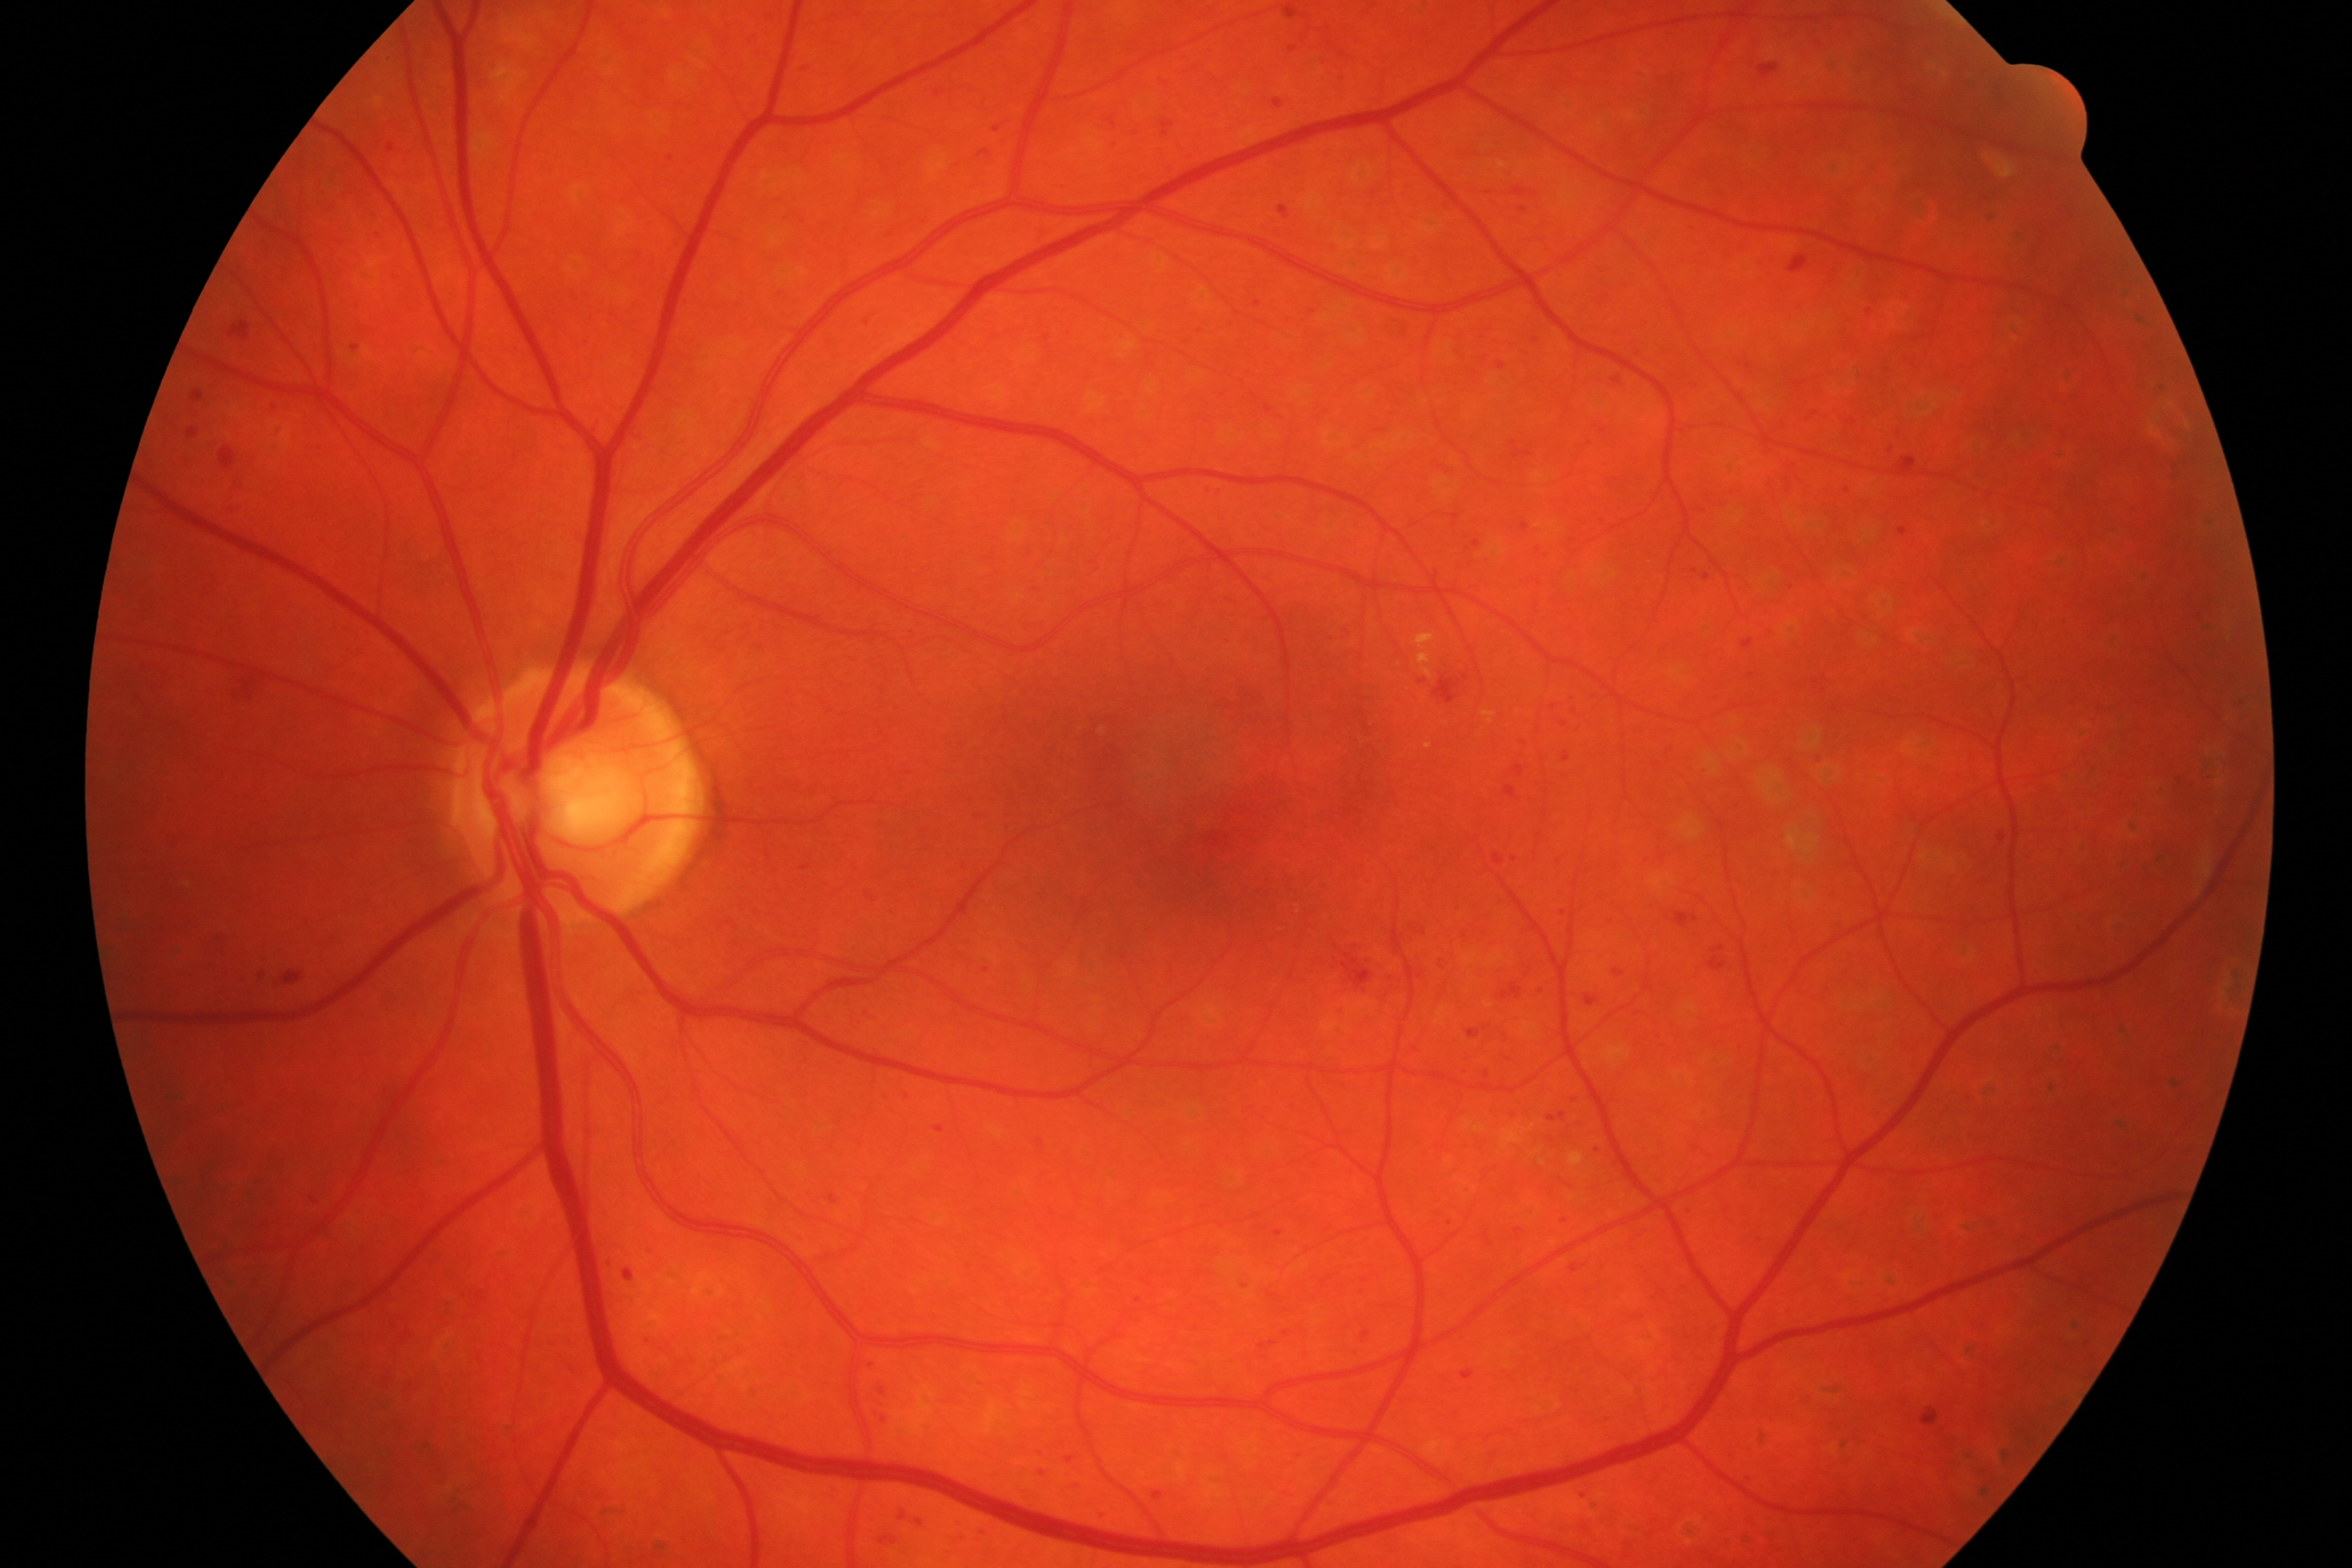
\includegraphics[width=\linewidth]{images/01_dr.jpg}
	\end{subfigure}
	\caption{Zużycie CPU dla sit funkcyjnych, dla 4 wątków; kolejne kody: 03, 04, 05}
\end{figure}
\begin{figure}[h!]
	\begin{subfigure}[b]{0.32\linewidth}
		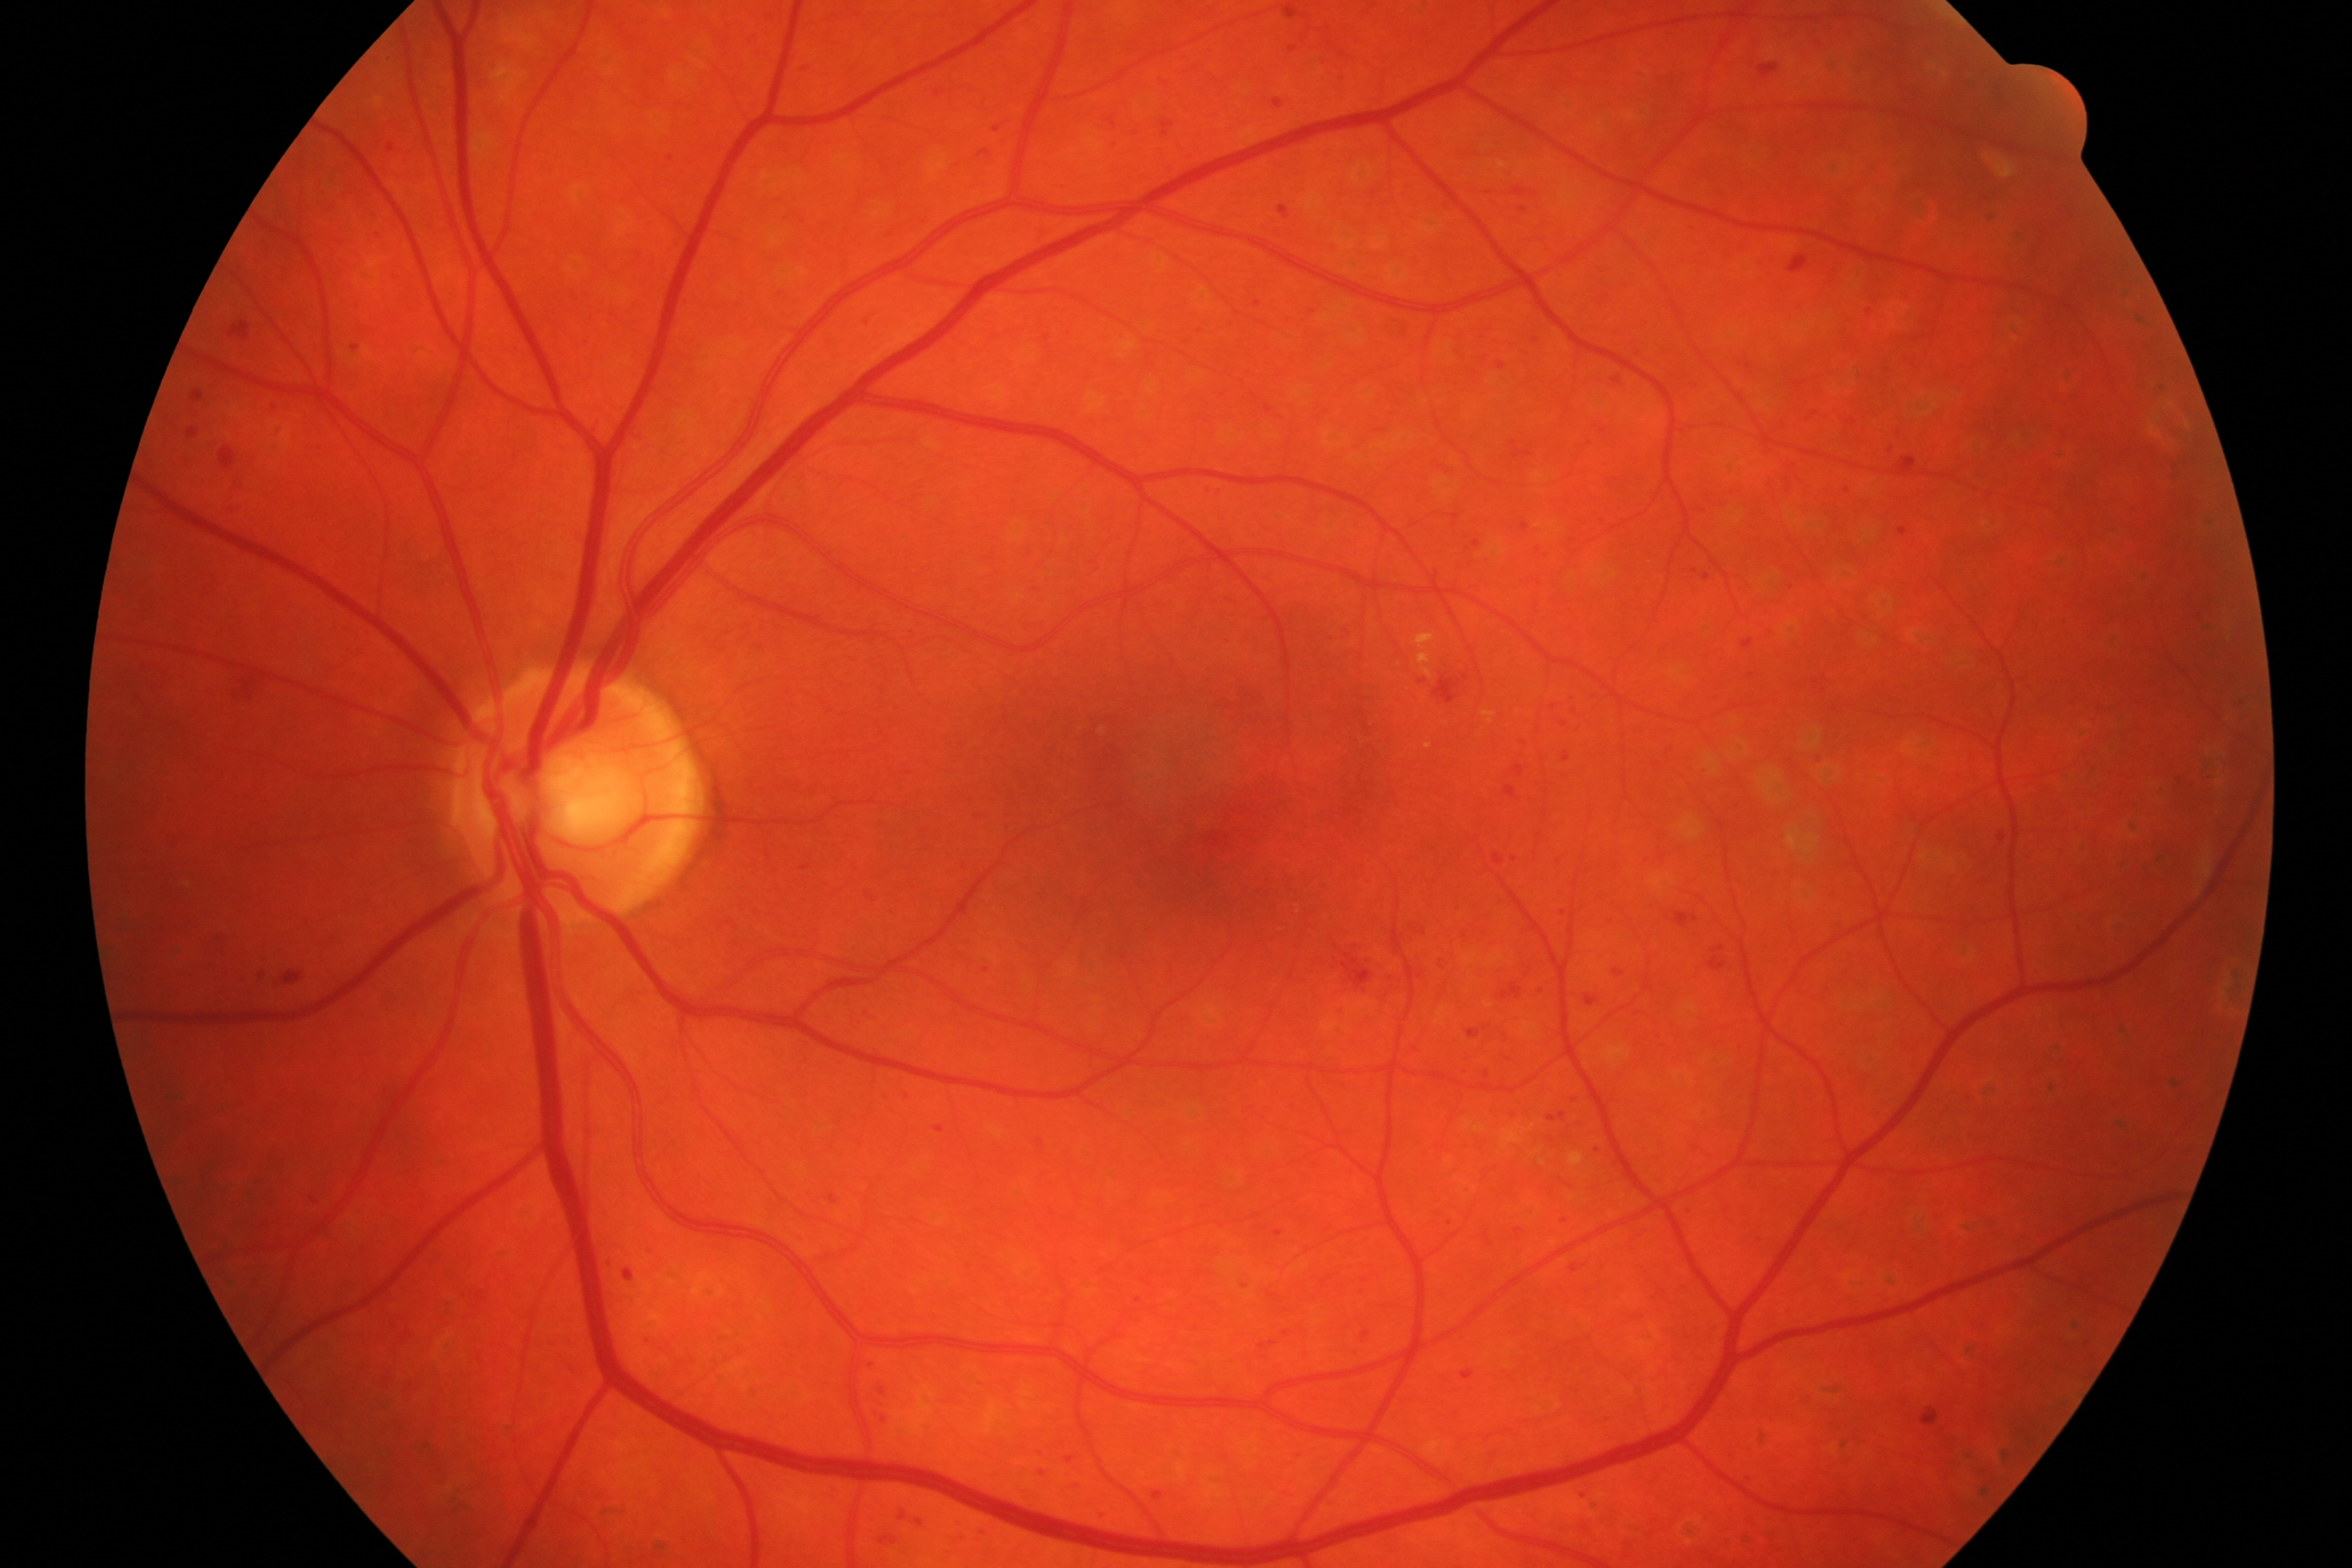
\includegraphics[width=\linewidth]{images/01_dr.jpg}
	\end{subfigure}
	\begin{subfigure}[b]{0.32\linewidth}
		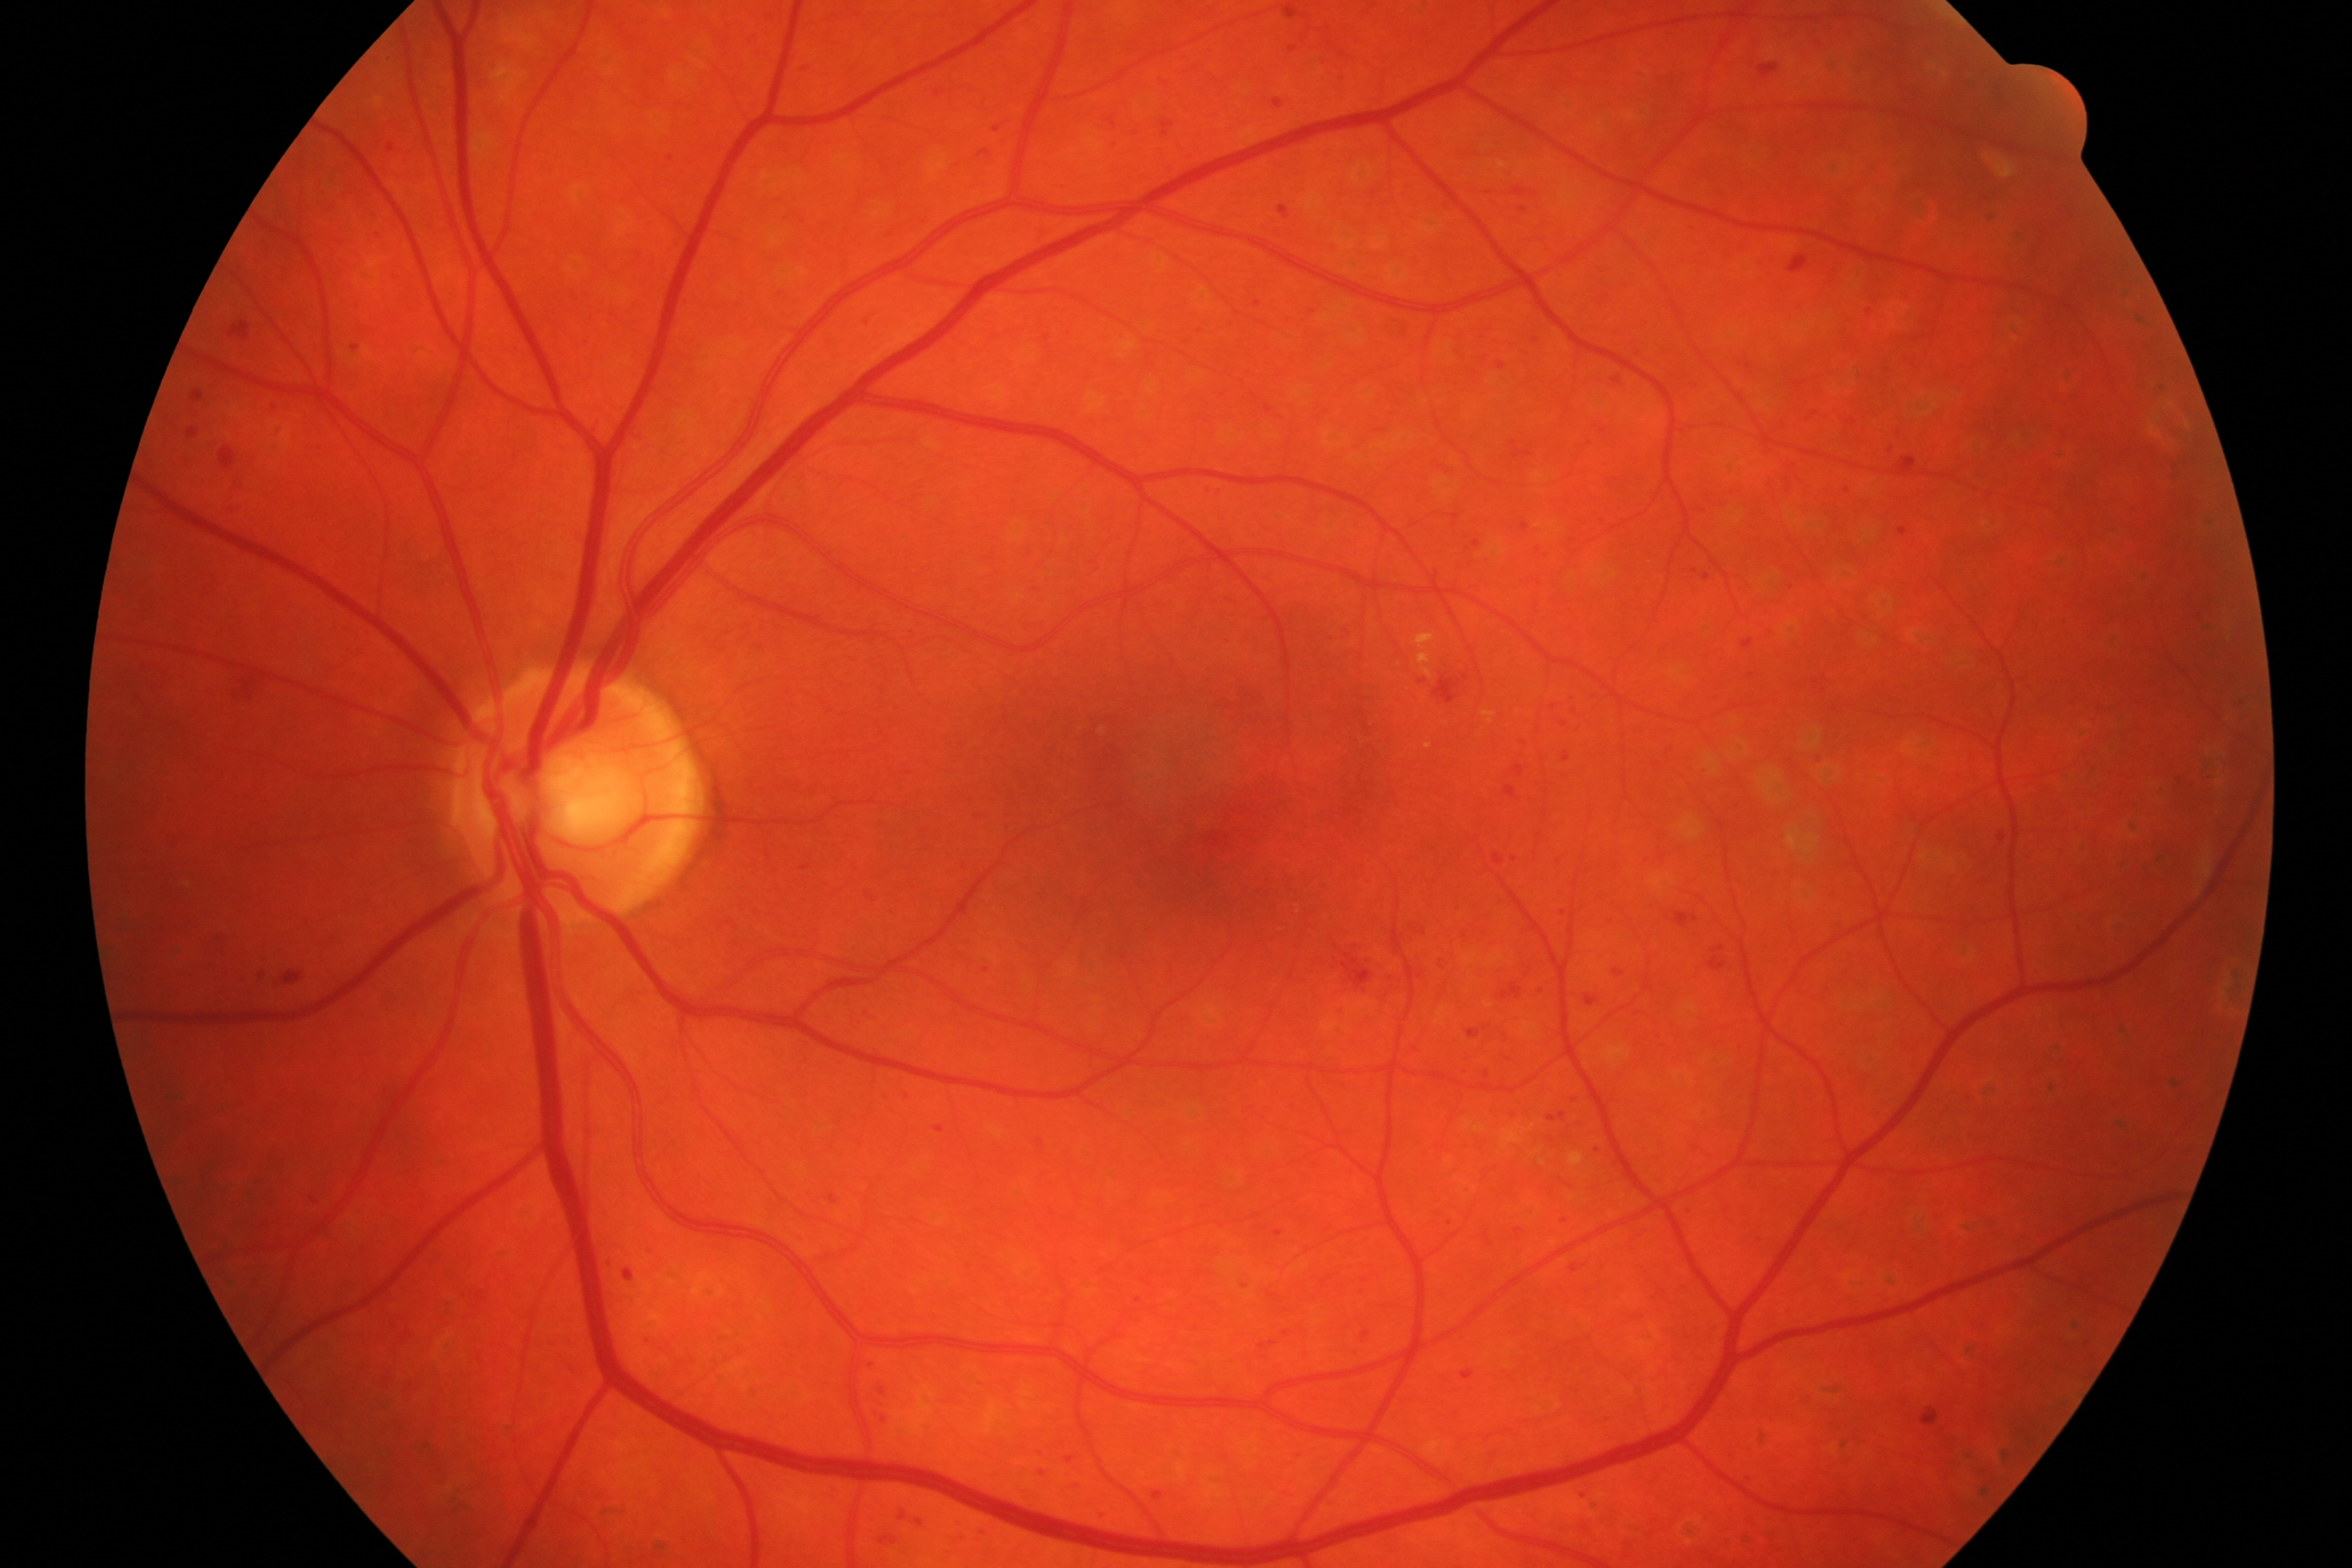
\includegraphics[width=\linewidth]{images/01_dr.jpg}
	\end{subfigure}
	\begin{subfigure}[b]{0.32\linewidth}
		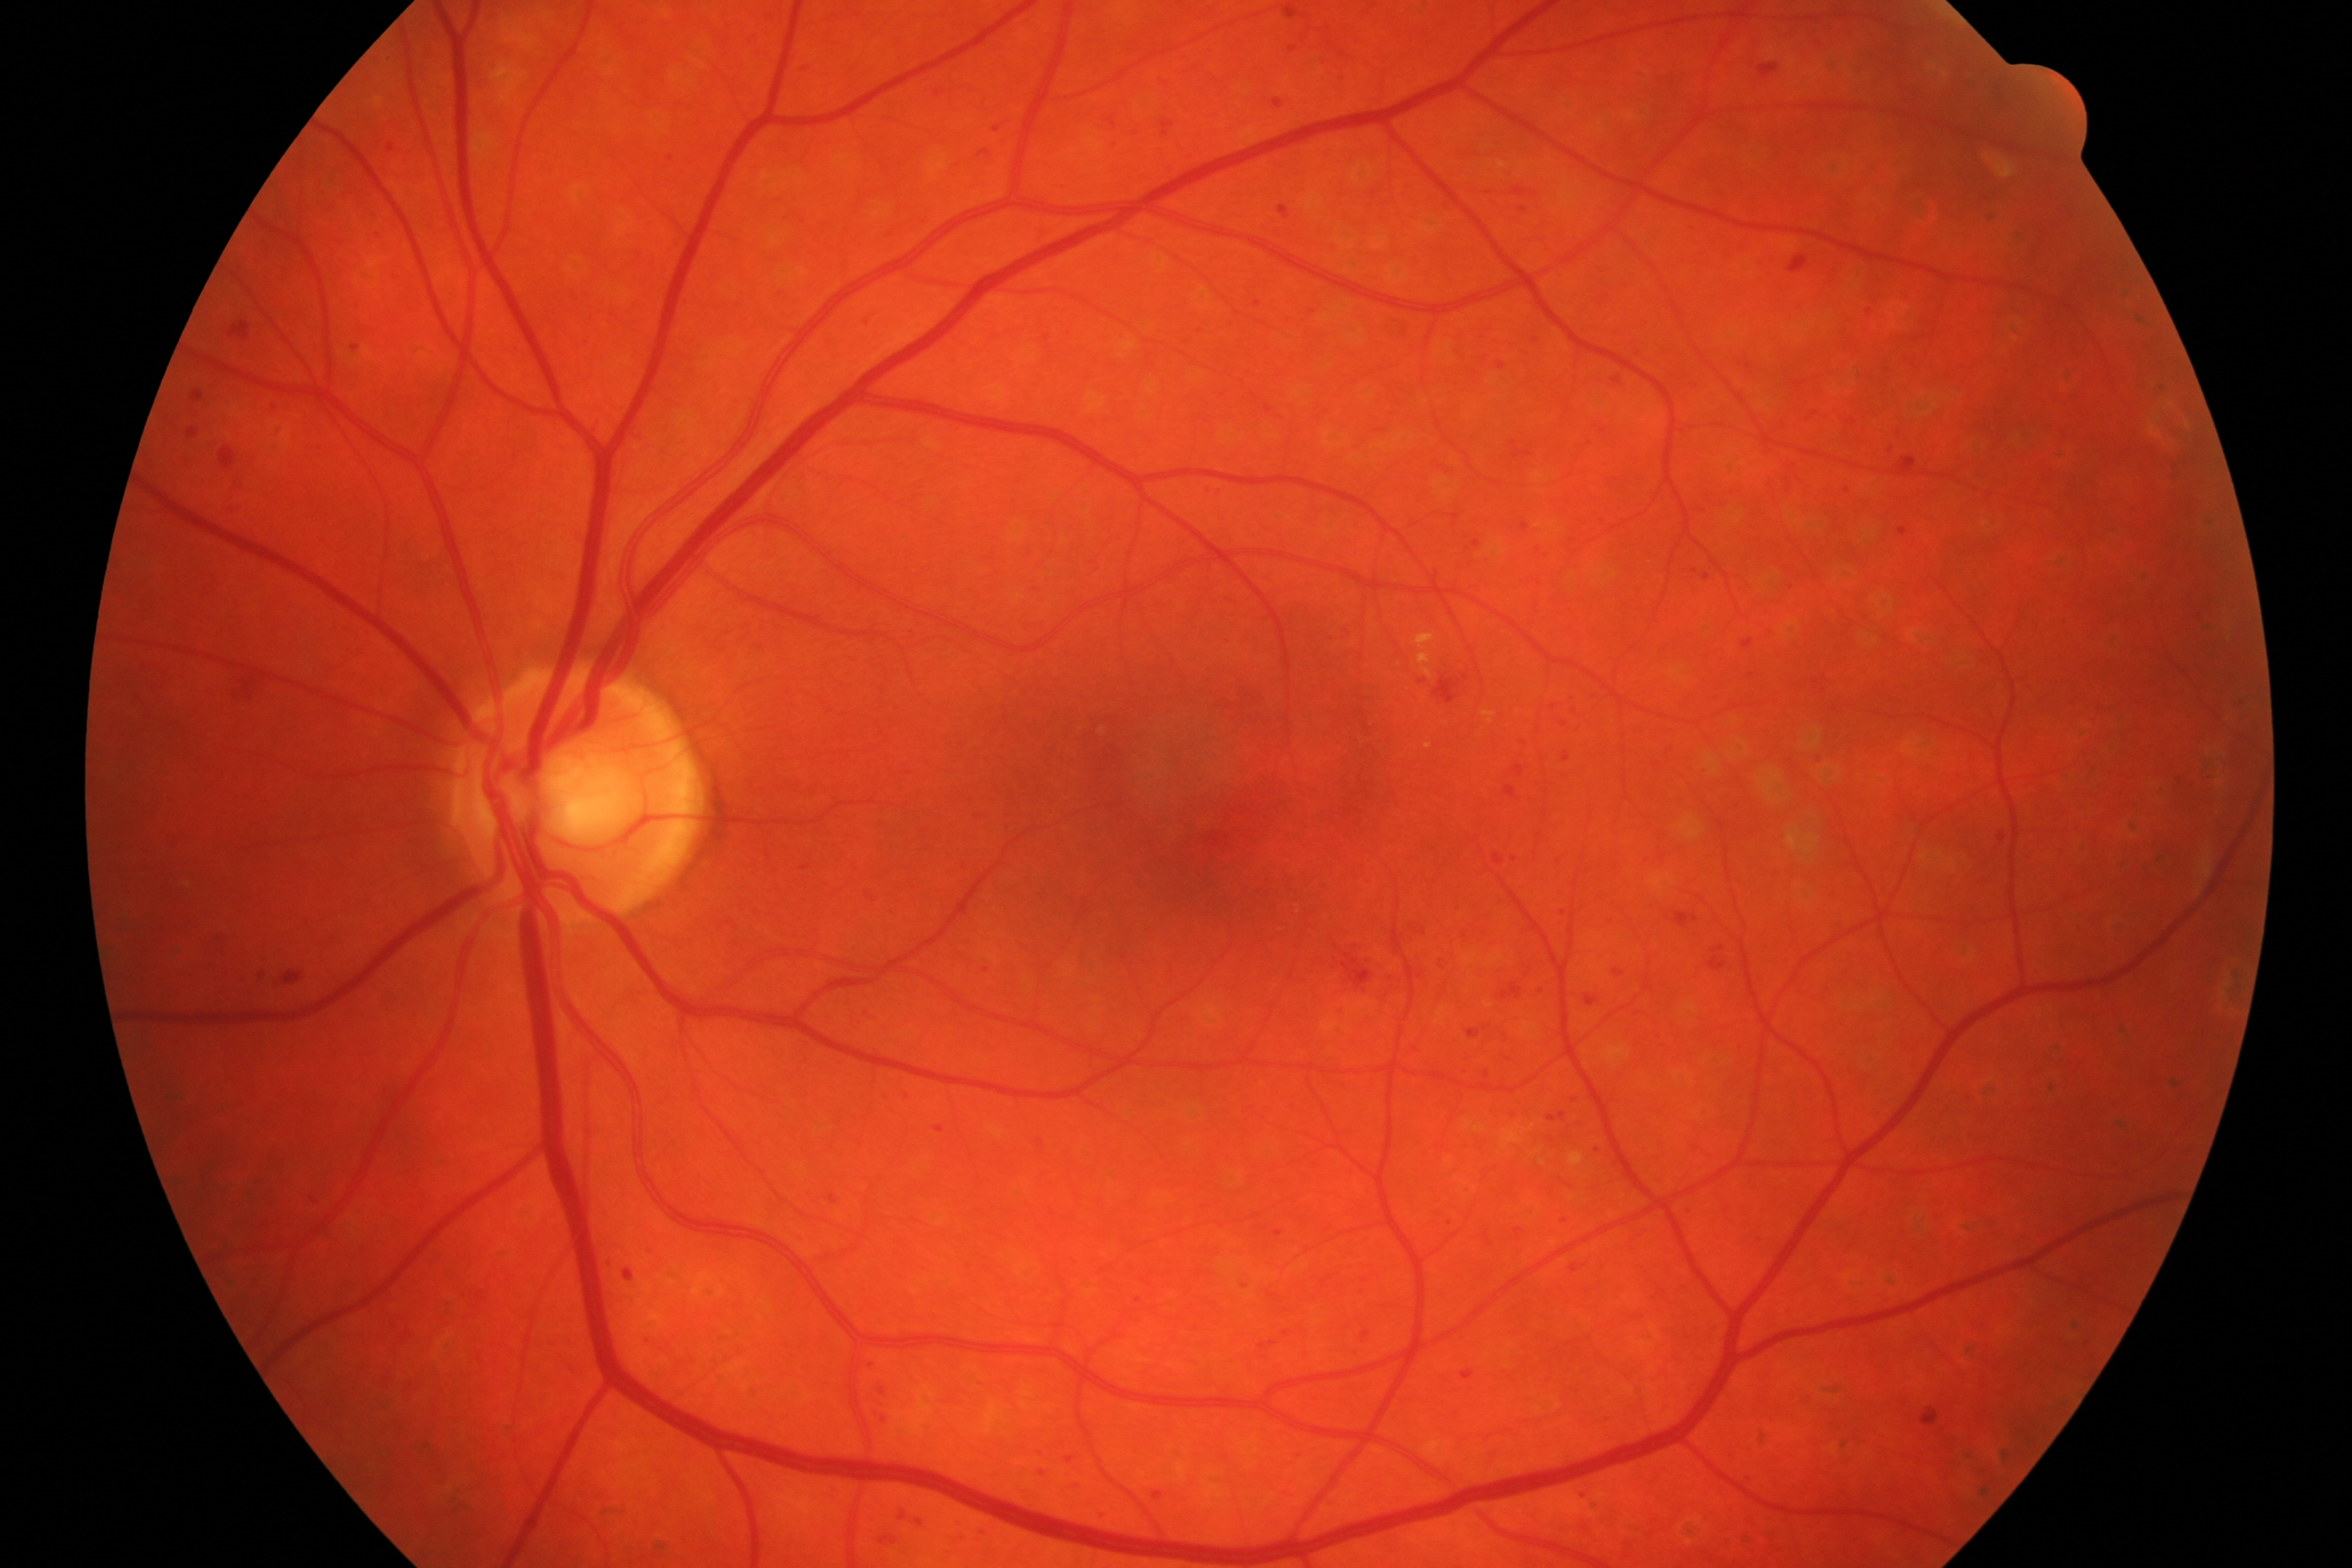
\includegraphics[width=\linewidth]{images/01_dr.jpg}
	\end{subfigure}
	\caption{Zużycie CPU dla kodu 07 używającego kolejno: 1, 2, 4 wątków}
\end{figure}
\begin{figure}[h!]
	\begin{subfigure}[b]{0.32\linewidth}
		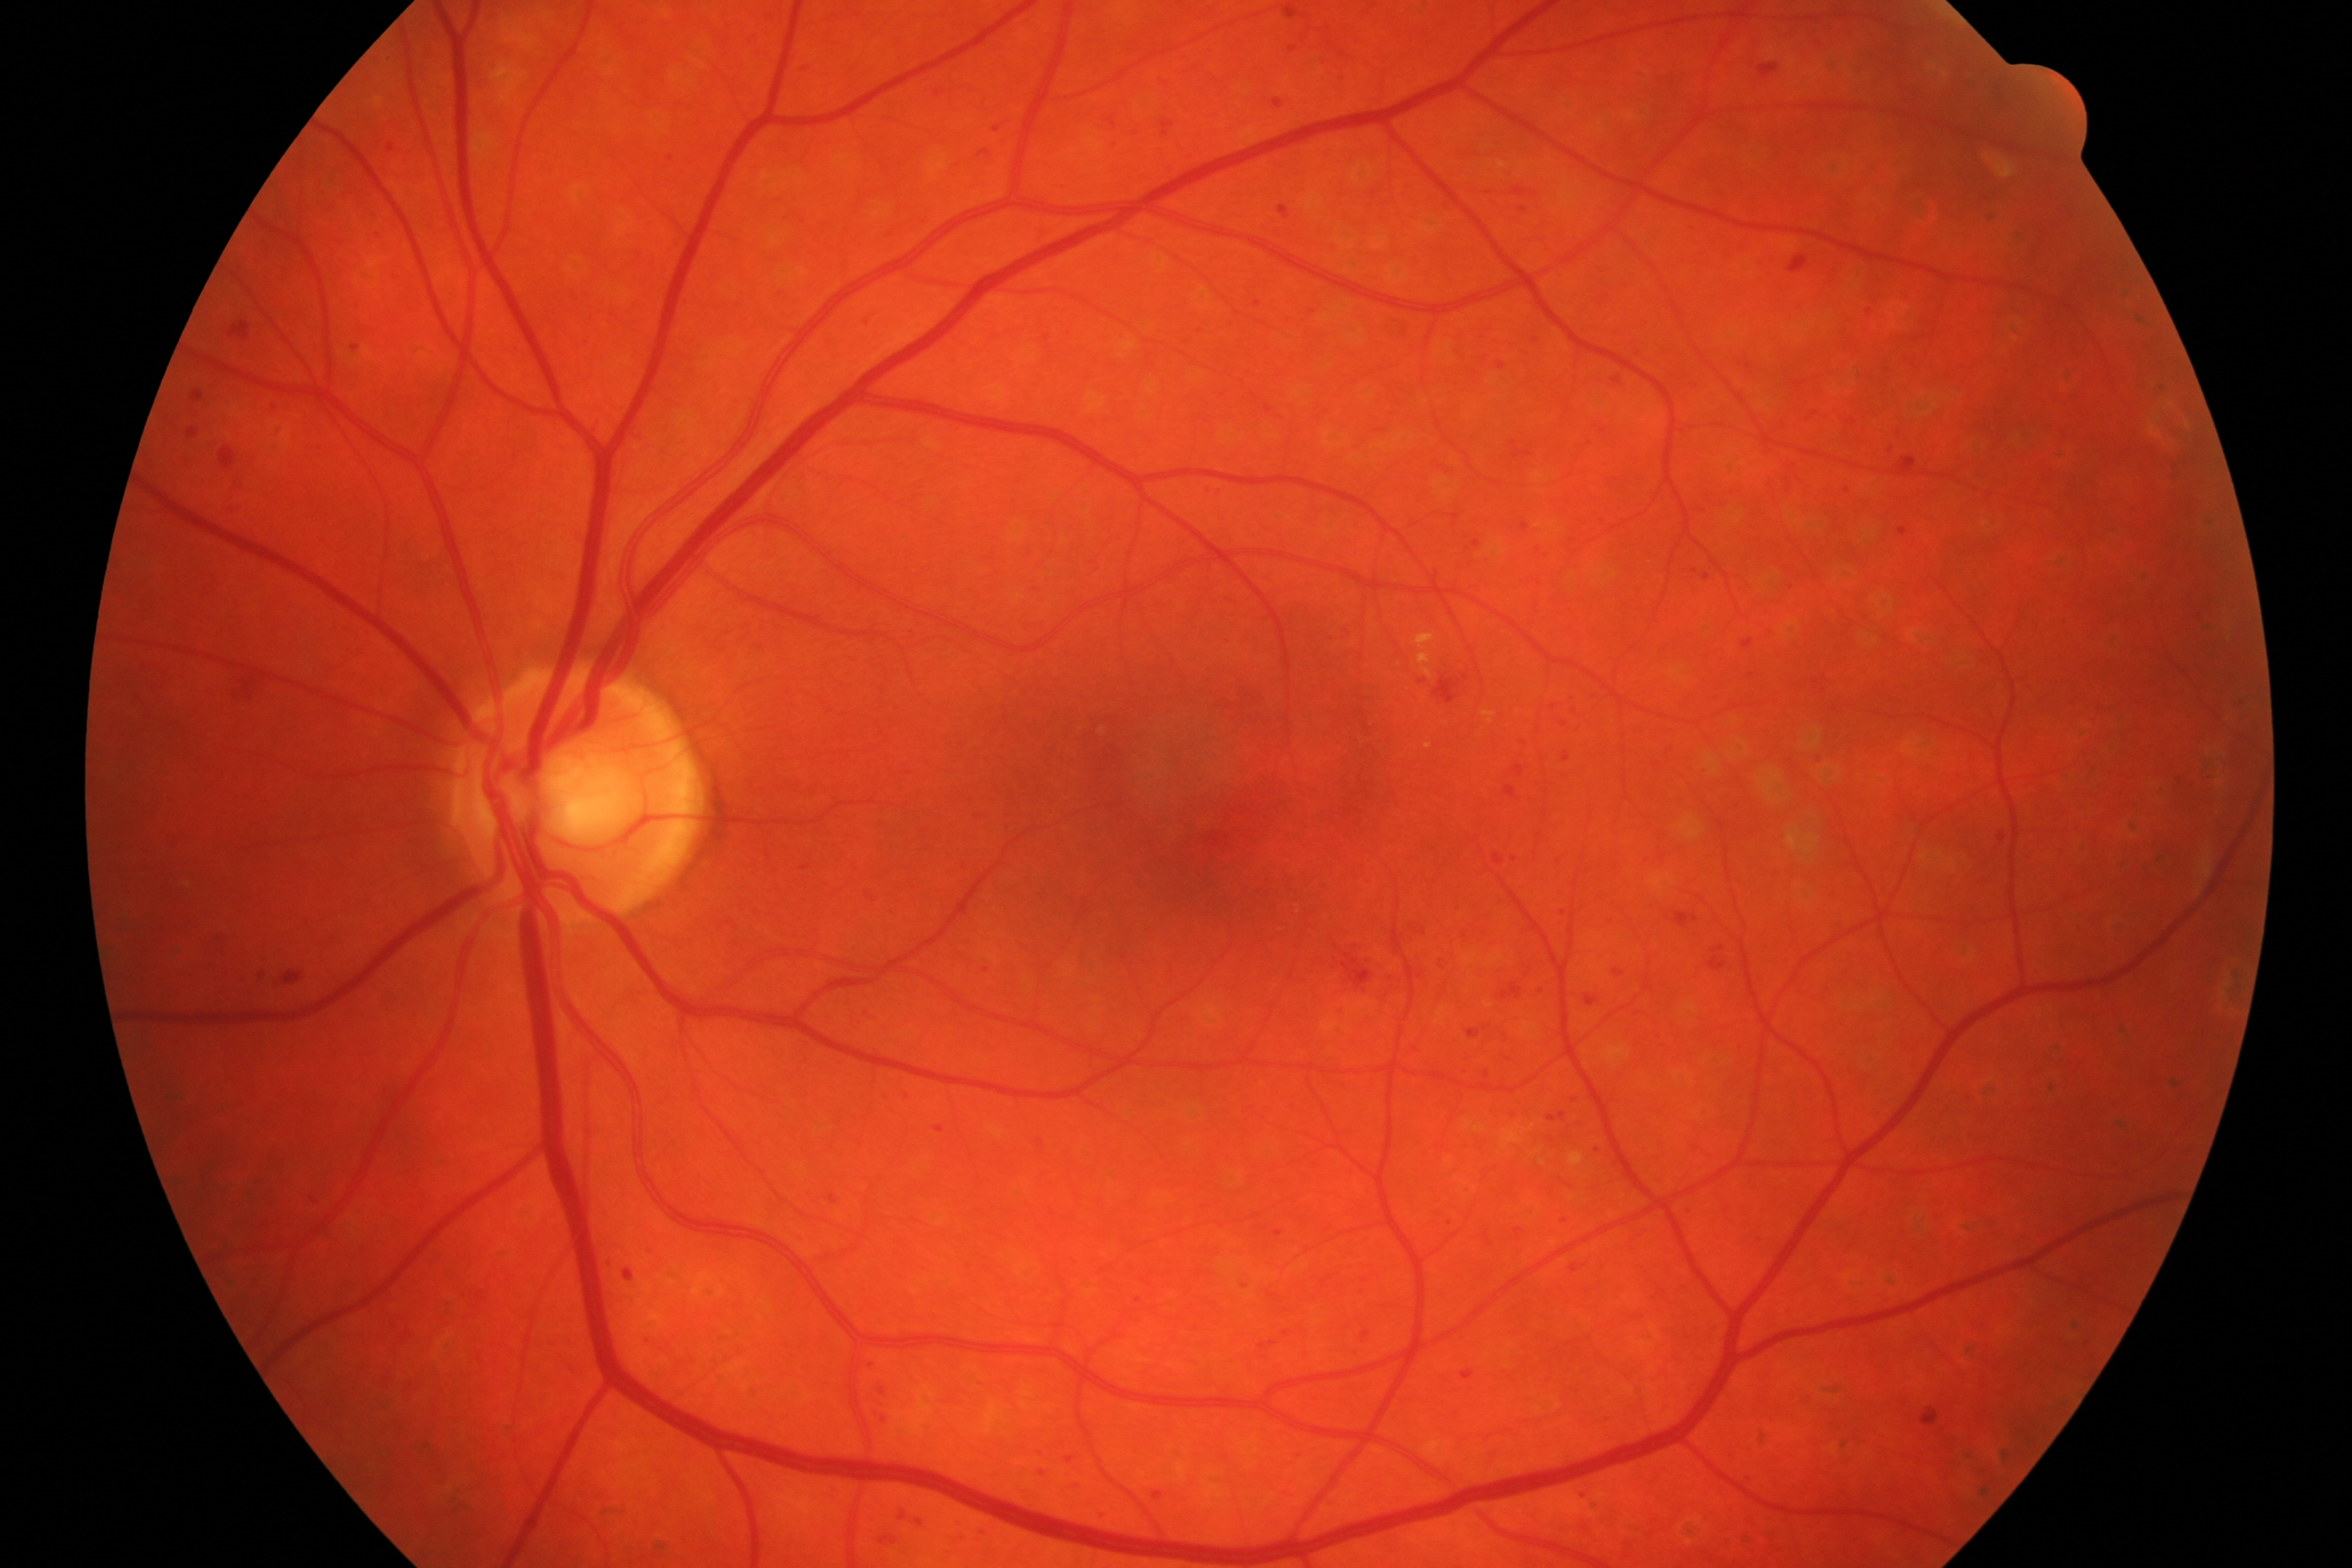
\includegraphics[width=\linewidth]{images/01_dr.jpg}
	\end{subfigure}
	\begin{subfigure}[b]{0.32\linewidth}
		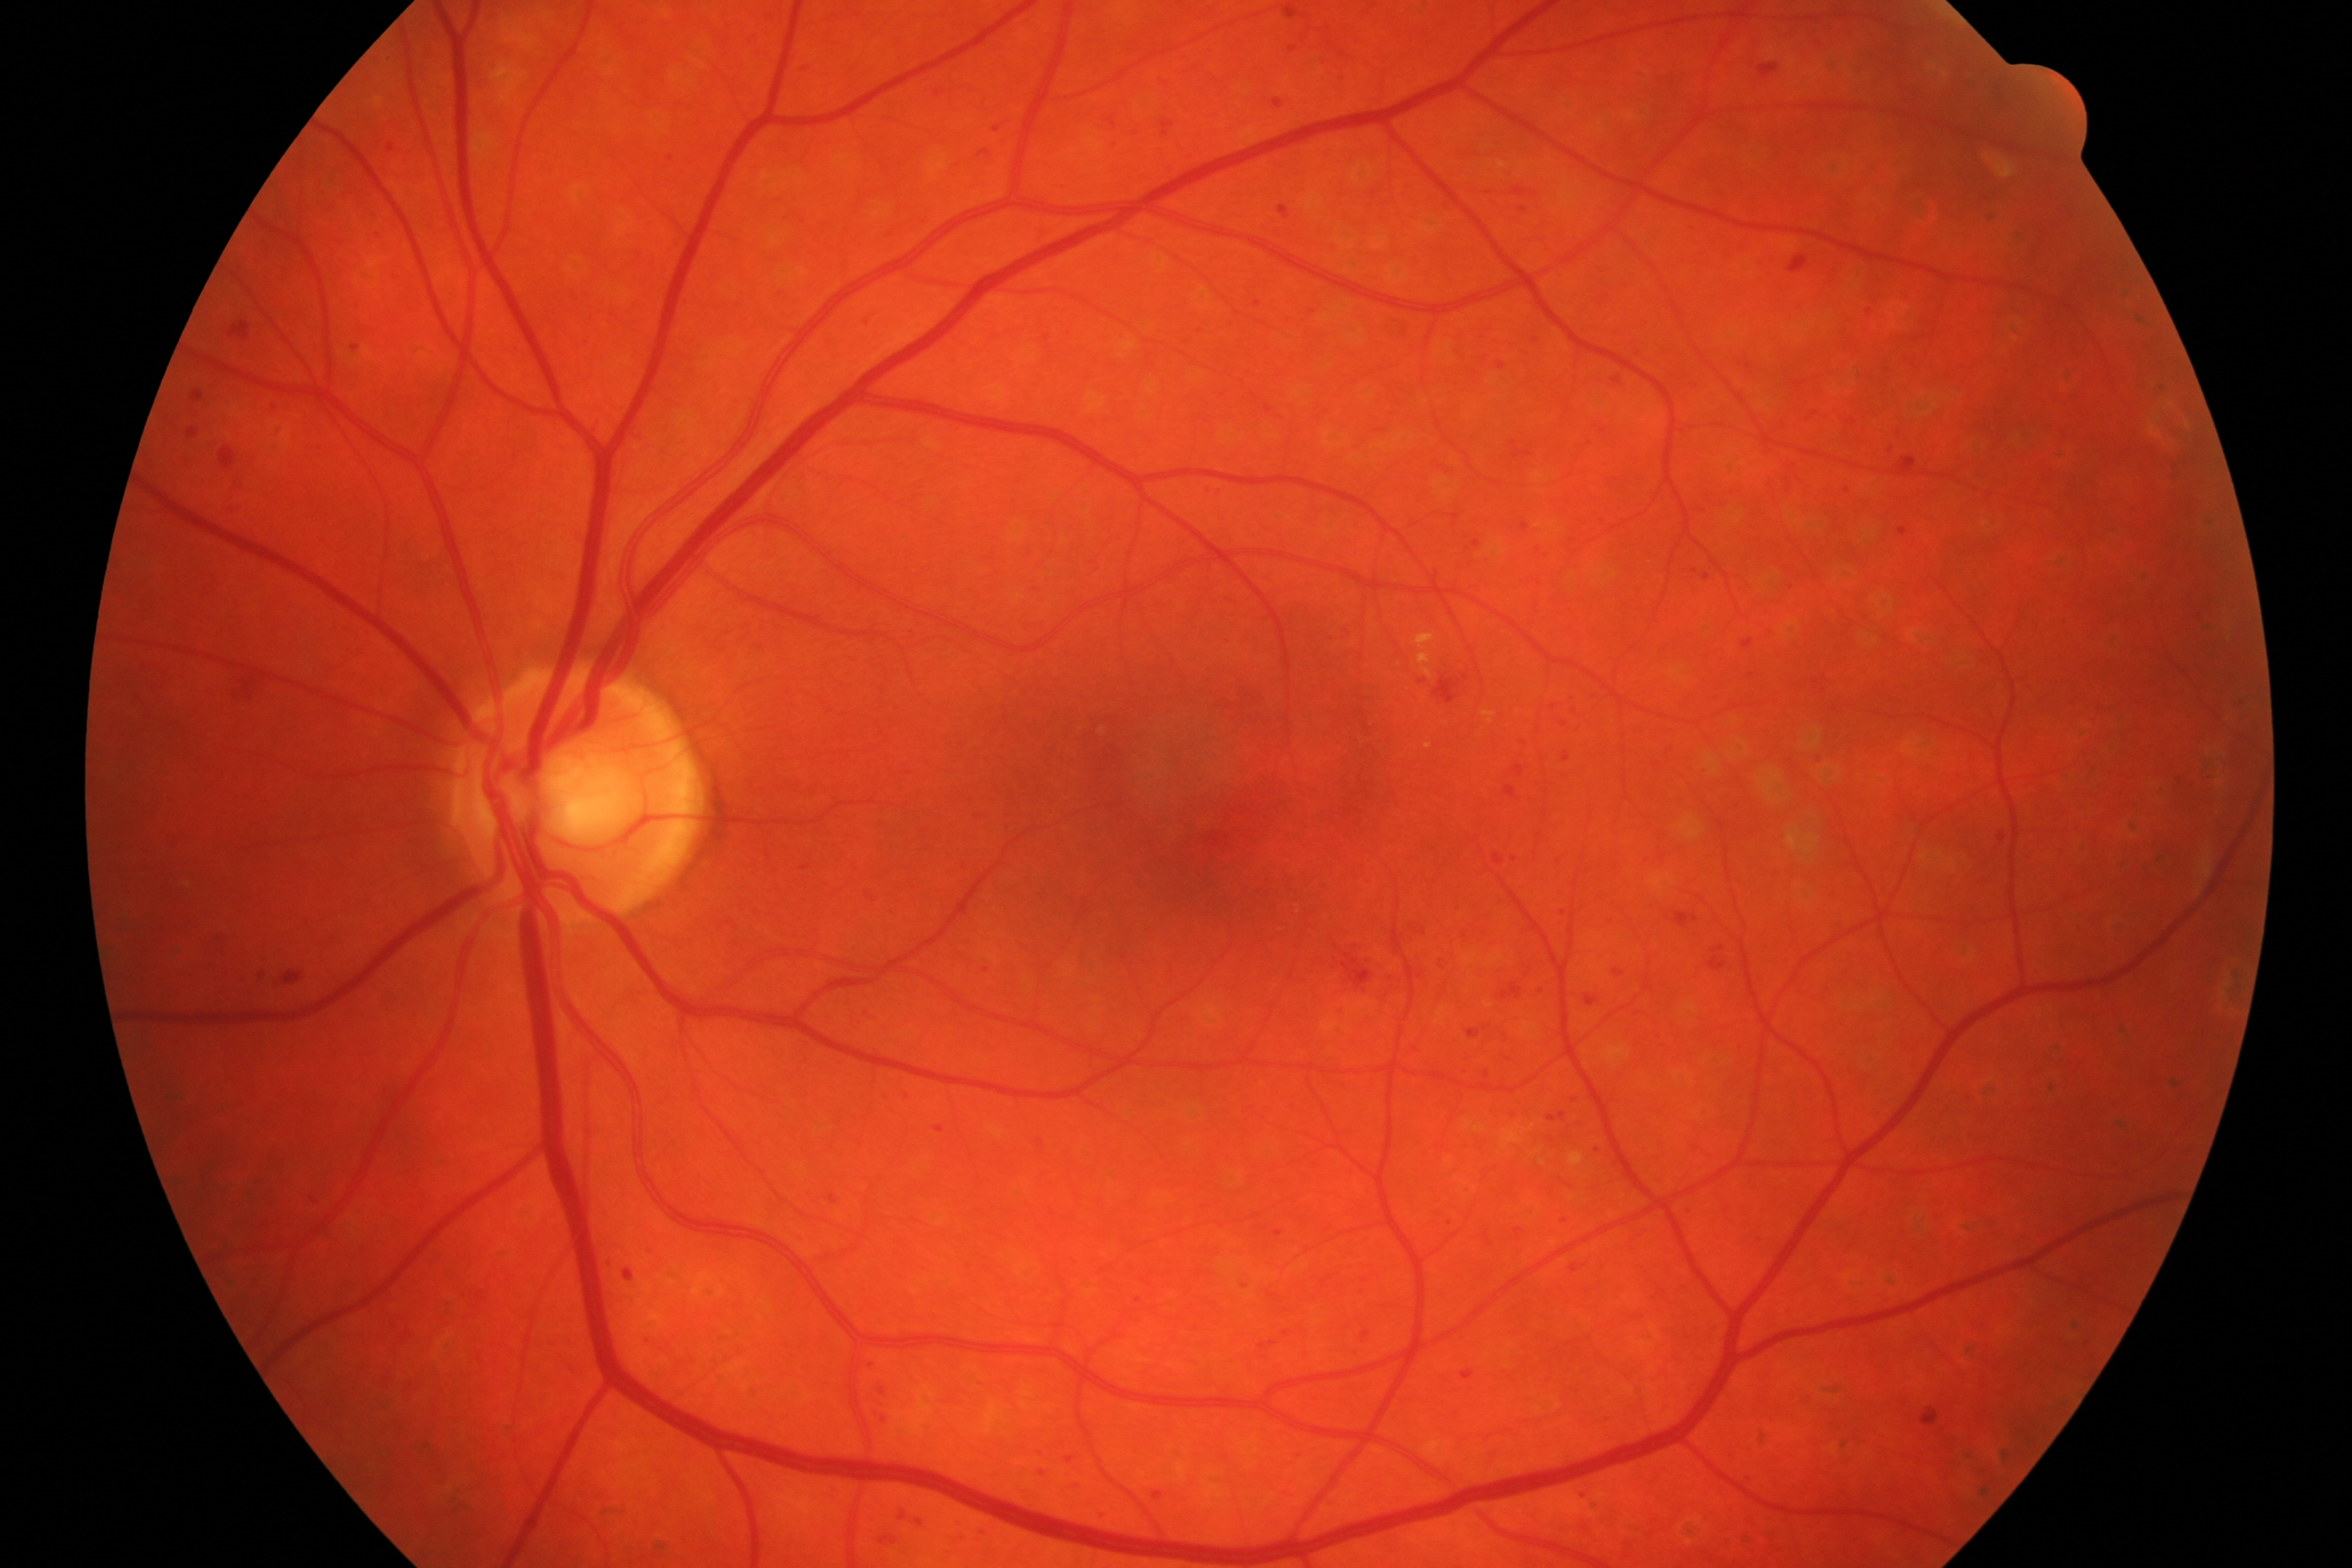
\includegraphics[width=\linewidth]{images/01_dr.jpg}
	\end{subfigure}
	\begin{subfigure}[b]{0.32\linewidth}
		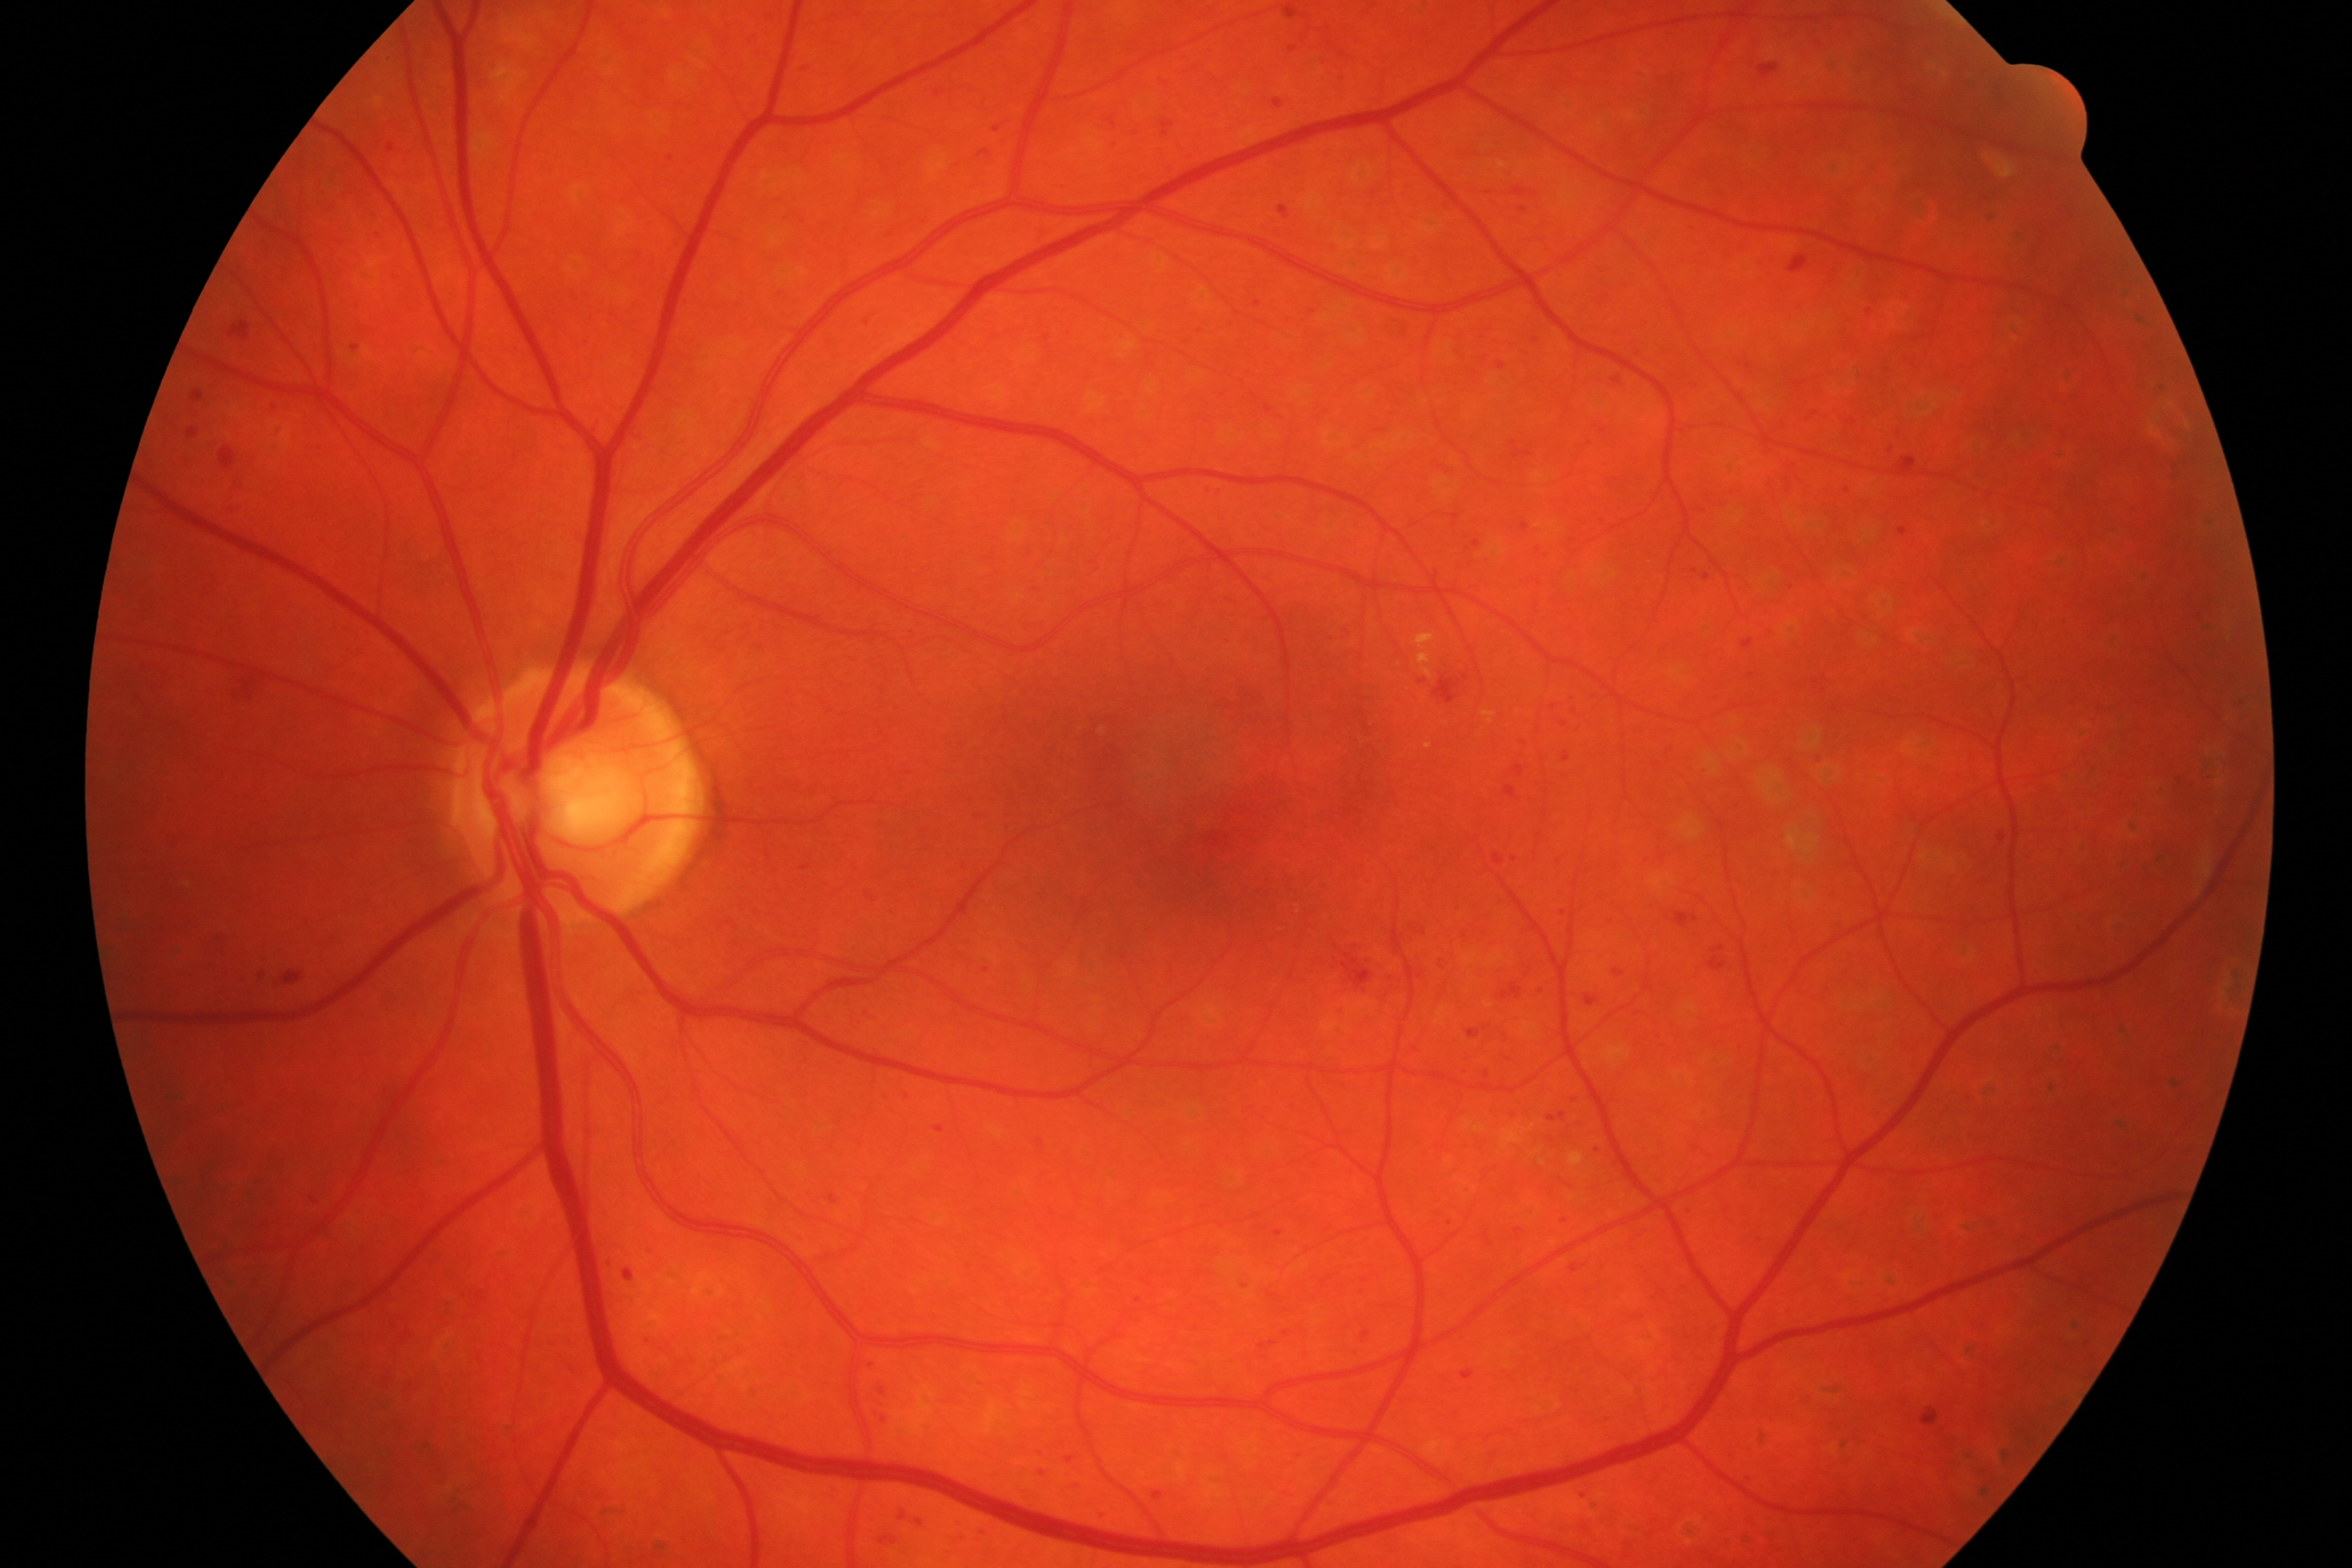
\includegraphics[width=\linewidth]{images/01_dr.jpg}
	\end{subfigure}
	\caption{Zużycie CPU dla kodu 08 używającego kolejno: 1, 2, 4 wątków}
\end{figure}

\section{Wnioski}
\begin{enumerate}

	\item Rozwiązanie oparte na wyznaczaniu dzielników mniejszych równych od \(\sqrt{n}\) bardzo efektywnie się zrównolegla - procesy dzielą się pracą bardzo równo, dla maksymalnej liczby wątków przez większość czasu działania programu wykonują się wszystkie wątki, ponieważ średnio jest używanych ponad 90\% zasobów procesora (dla maksymalnej liczby 4 wątków). Zwiększenie liczby procesów \(k\)-krotnie powoduje zmniejszenie czasu przetwarzania prawie \(k\)-krotnie (dla \(k=4\) zachodzi ponad \(\frac{7}{2}\)-krotne zwiększenie wydajności), przy założeniu, że nowy wątek jest wykonywany przez inny procesor logiczny. Nie zachodzi prawie wcale False Sharing, ponieważ jedyna współdzielona zmienna to tablica liczb pierwszych. Wątki nie czytają współdzielonej pamięci, co powoduje, że bardzo rzadko zachodzą cache missy - wynika to z niskiego Memory Bounda, 9-krotnie niższego niż w sekwencyjnym sicie. Wąskim gardłem rozwiązania jest Front-End Bound, najwyższy spośród wszystkich (poza 08) rozwiązań - co oznacza, że są większe problemy z dostarczeniem zadania do wykonania do Back-endu niż z jego wykonaniem; a także intensywne dzielenie, zwiększające Core-Bound. Algorytm pomimo zrównoleglenia nadal jest wolniejszy od sekwencyjnego sita, ponieważ ma większą złożoność - dla \(n=10^9\) ponad 10-krotnie wolniejszy, dlatego nie został uwzględniony w sprawozdaniu z maksymalnymi wartościami \(l, r\).

	\item Sito Erastotenesa w podejściu funkcyjnym było w stanie uzyskać około \(\frac{2}{3}\) czasu działania sekwencyjnego sita używając dynamic schedulingu (Kod 05, linia 51). Co ciekawe, rozwiązania używające handmade schedulingu (kod 04) jest około \(\frac{1}{9}\) razy wolniejsze od rozwiązania używającego dynamic schedulingu (dla 4 rdzeni), co jest skorelowane z współczynnikiem "effective physcial core utilization" - wynika stąd, że sito używające dynamic schedulingu pomimo narzutu związanego z synchronizacją nadal jest szybsze od ręcznego przydziału liczb do procesów, który nie przydzielał perfekcyjnie procesów do zadań, co widać na 1. obrazku. Wskazuje to na niedoskonałość heurystyki, której użyto - nie uwzględniono cache procesora - procesy, które będą skreślać niskie liczby, częściej będą zaliczały trafienie w lokalnym cache. Obserwacja ta została wykorzystana do konstrukcji kodu 08. Zgodnie z oczekiwaniami, kod używający statycznego przydziału iteracji do procesu ma bardzo niski współczynnik efektywnego użycia cpu - dla 4 wątków prawie 3 razy niższy niż ten z dynamic schedulingiem. Co ciekawe, kod ten ma też mniejszy o 2 punkty procentowe Memory Bound niż 2 pozostałe sita w podejściu funkcyjnym - wynika to z mniejszej ilości cache missów, jako że tylko jeden wątek ma dla siebie całe cache przez większość czasu trwania programu.
	
	\item Efektywność standardowego sita domenowego pozostawia wiele do życzenia - jest ono około \(\frac{2}{7}\) razy wolniejsze od sita funkcyjnego z dynamic schedulingiem dla tej samej liczby wątków; problem wydajnościowy zapewne tkwi w zarządzaniu pamięcią; z zebranych danych wynika, że ten algorytm jako jedyny blokował się częściej niż 0.1\% razy na przedziale alokacji, mając znaleziony segment pamięci w DRAMie. Algorytm ponadto miał większy narzut związany z core boundem - najprawdopodobniej wynika to z intensywnego używania slotów procesora. Z danych można wyciągnąć wniosek, że algorytm użytkował wszystke procesory w miarę równomiernie, jednak zwiększenie liczby procesorów nie powoduje zmniejszenia czasu przetwarzania o więcej niż \(\frac{1}{12}\). Wszystkie te dane i natura algorytmu skłaniają do sformułowania wniosku: kod sita domenowego jest wolny w porównaniu do funkcyjnych, ponieważ procesy zapełniają globalny cache własnymi częściami sita, a jako że każdy wątek ma inny segment, te części pamięci się nie pokrywają, często zachodzą Cache Missy, co spowalnia algorytm mimo nieomal pełnego wykorzystania procesorów. Problem ten nie zachodzi w takim wymiarze dla sita funkcyjnego, ponieważ segmenty pamięci mogą się pokrywać, co za tym idzie częściej zajdzie cache hit, a false sharing nie jest dużym narzutem na efektywności powyższych kodów. Aby sprawdzić zasadność tej tezy, stworzony został kod super-sita domenowego z przesuwaniem o liczbę niższą niż ilość danych, która zmieści się w L1 cache jednego rdzenia procesora - kod ten powinien być znacznie szybszy i efektywnie zmniejszać czas trwania przetwarzania.
	
	\item Najbardziej efektywne jest ulepszone sito domenowe - zrównolegla się bez żadnego problemu (dla \(k\) wątków i \(t_{sequential} =\) czas dla 1 wątku, czas przetwarzania to \(\frac{t_{sequential}}{k}\) - rysunek 3. pokazuje, jak efektywnie wykorzystywano rdzenie procesora), a czas przetwarzania dla 1 wątku jest 7 razy krótszy niż czas przetwarzania standardowego sita. Wynika to z zapewnienia tego, że większość operacji w pamięci zaliczy trafienie już na etapie L1 cache - nie wynika to z pojedynczej linii, ale z konstrukcji algorytmu i iterowania się w batchach co 32000 intów, czyli 128.000 bajtów, które mogą się zmieścić w L1 cache. Ponadto sam algorytm nie generuje dużo większego narzutu niż zwykłe sito, chociaż złożoność ma uzależnioną od liczby, o którą się przesuwam - jeśli można ją oszacować przez co najmniej \(O(\sqrt{n})\) dla \(n\)- rozmiaru sita, to sito wykona co najwyżej \(O(\sqrt{n})*O(\sqrt{n})=O(n)\) "pustych przelotów" - iteracji, w trakcie których nie przejdę do skreślania liczb pierwszych (ponieważ liczba liczb pierwszych \(p\le\sqrt{n}\) jest ograniczona przez \(\sqrt{n}\), a liczba iteracji przez odwrotność przesunięcia sita pomnożoną przez rozmiar sita - czyli \(O(\sqrt{n})\). To ogranicza złożoność algorytmu do złożoności standardowego sita. Procesy nadal dzielą między sobą po równo liczbę elementów części otwartej sita, co za tym idzie algorytm jest najlepszy zarówno w kontekście zrównoleglania, jak i efektywności.
	
	\item W większości rozwiązań dominują ograniczenia pamięciowe, związane z wysokim Memory Boundem, pomiędzy 70\% a 80\% - w tych kodach procent przedziałów alokacji, które zostały zatwierdzone jest niższy niż 10\%. Wyjątkami są kody 09 i 08. Zarówno w kodzie opartym na intensywnym dzieleniu (09), jak i w kodzie ulepszonego sita domenowego (08) ograniczenia związane z front-end boundem są zbliżone, a czasem nawet wyższe od ograniczeń związanych z back-endem, w tym pamięcią.
	
	\item Jedynie kod 08 był wiele efektywniejszy od pozostałych kodów (ponad 24 razy szybszy niż sekwencyjny na 4 rdzeniach). Kod ten miał nieomal niezmienną efektywność (pomiędzy 6 a 7) niezależnie od liczby procesów, w przeciwieństwie do standardowego sita domenowego (07) - które traciło na efektywności przy wzroście liczby procesów mimo wykorzystania procesora rzędu 95\%. Kody funkcyjne także traciły na efektywności razem ze wzrostu liczby używanych wątków, w efekcie ich przyspieszenie względem sekwencyjnego kodu nie wzrastało do wartości wyższych niż 2.
\end{enumerate}

\section{Podsumowanie}
	Celem tego projektu było przedstawienie efektywnego algorytmu równoległego do znajdywania liczb pierwszych w przedziale. Cel ten został zrealizowany w kodzie 08, pozostałe pokazywały pewne własności przetwarzania równoległego, które naprowadzały na sposób realizacji tego celu. Można także zastosować podobną optymalizację dla wersji funkcyjnej kodu, ale aby uzyskać satysfakcjonującą prędkość przetwarzania należałoby aktualizować 4 tablice - to redukuje problem false sharingu. Problemem z tym rozwiązaniem jest brak dostępnej pamięci - należałoby zaalowkować jej ~5 GB, co nie jest możliwe na używanym do realizacji zadania sprzęcie.

\end{document}
